\documentclass{book}
\usepackage[utf8]{inputenc}
\usepackage[spanish]{babel}
\usepackage{amsmath,amssymb,amsfonts} %Fonts de AMS
\usepackage{mathbbol} %Font para matrices como la identidad
%%Formato de hoja%%
\usepackage[margin=1.5cm]{geometry}

%%Imagenes%%
\usepackage{graphicx}
\usepackage{wrapfig}
\usepackage{caption}
\usepackage{subcaption}
\graphicspath{{./fig/}}
\usepackage{float}

%%Ecuaciones y teoremas
\numberwithin{equation}{section} %Número de ecuación por sección

\newtheorem{definition}{Definición}[chapter]
\newtheorem{axiom}{Axioma}[chapter]
\newtheorem{law}{Ley}[chapter]
\newtheorem{principle}{Principio}[chapter]
\newtheorem{postulate}{Postulado}[chapter]
\newtheorem{collorary}{Colorario}[chapter]
%\setcounter{\thelaw}{0}

\title{Resumen de Física 4}
\author{S. Schiavinato}
\date{}

\begin{document}
\maketitle

\chapter{Termodinámica}
\section{Definiciones básicas}

\begin{definition}[Sistema]
    \begin{figure}
    \centering
    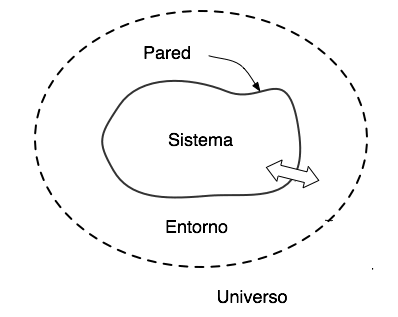
\includegraphics[width=0.6\textwidth]{termodinamica_sistema}
    \caption{Representación gráfica de un sistema termodinámico}
    \label{fig:termodinamica_sistema}
    \end{figure}
\end{definition}

\begin{definition}[Variables termodinámicas]
Son propiedades o magnitudes físicas necesarias para describir el proceso a estudiar.
\begin{itemize}
\item Extensivas $X_i$
\item Intensivas $Y_i$
\end{itemize}
\end{definition}

\begin{definition}[Estado] 
    Conjunto de variables bien definidas del sistema
\end{definition}


\begin{definition}[Equilibrio]
El estado del sistema no cambia en el tiempo
\end{definition}


\begin{principle}[Existencia de los estados de equilibrio]
Existen los estados de equilibrio para sistemas caracterizados por finitas variables termodinámicas extensivas.
\end{principle}


\begin{law}[Cero: Transitividad del equilibrio]
\end{law}

\section{Primera Ley}
\begin{figure}[H]
\centering
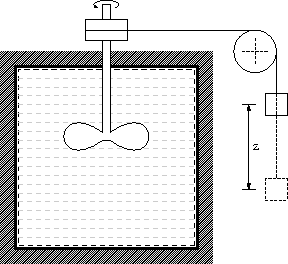
\includegraphics[width=0.35\textwidth]{primera_ley}
\caption{Experiencias de Joule}
\label{fig:primera_ley}
\end{figure}
\begin{definition}[Energía interna]

\begin{equation}
dU = - d'W_{ad}
\end{equation}

\begin{equation}
\oint dU = 0
\end{equation}

\end{definition}


\begin{law}[Primera: Conservación de la energía]

\begin{equation}
\Delta U = Q - W \implies dU = \delta Q - \delta W
\end{equation}

\end{law}


\subsection{Trabajos generalizados}

\begin{definition}[Trabajo generalizado]

\begin{equation}
d'W = \sum_i Y_i dX_i
\end{equation}
con $Y_i$ una variable intensiva y $X_i$ una variable extensiva

\end{definition}

\section{Segunda ley}
\begin{law}[Enunciado de Kelvin]
No es posible tener una máquina térmica ciclica que tenga como único resultado eliminar calor de una fuente y transformarlo en trabajo.
\end{law}
De este principio nos queda definir que es una máquina térmica ciclica
\begin{definition}[Maquina térmica ciclica]
\begin{figure}[H]
    \centering
    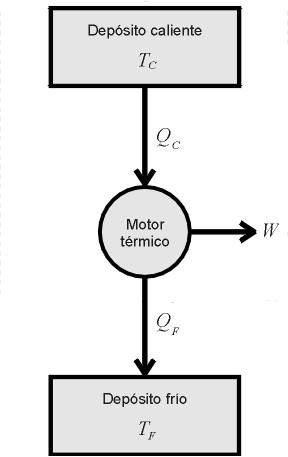
\includegraphics[width=0.19\textwidth]{motor}
    \caption{Esquema simbólico del motor térmico}
\end{figure}
\end{definition}


\begin{collorary}[Existencia de la entropía]
 $\exists S = S(U, \{X_i\})$, (en particular $U$, $V$ y $N$), tal que  $dS = 0 \implies \delta Q = 0$.
\end{collorary}

\begin{figure}[H]
\centering
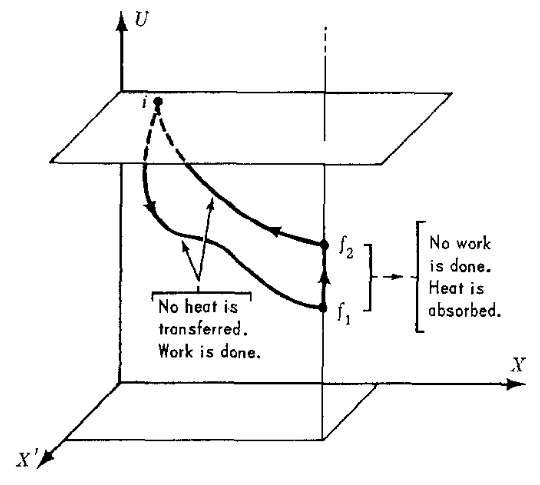
\includegraphics[width=0.6\textwidth]{segunda_ley_espacio}
\caption{Diagrama del argumento para seleccionar puntos inalcanzables por transformaciones adiabáticas}
\label{fig:segunda_ley_espacio}
\end{figure}

Esas superficies las vamos a parametrizar con \[S(U,\{X_i\}) = c,\] siendo S una función continua suave (ya que asumimos que las superficies son suaves).

\[S(U,\{X_i\}) = c \implies \delta Q = 0\]
Por lo tanto tengo
\[dU = \frac{\partial U}{\partial S} dS + \frac{\partial U}{\partial X_i} dX_i = \delta Q - \delta W\]
ergo
\begin{equation}
\delta Q = \frac{\partial S}{\partial U} dS = \lambda dS
\end{equation}

Elegimos $\lambda$ tal que
\begin{equation}
\frac{1}{T} = \left.\frac{\partial S}{\partial U}\right|_{X_i}
\label{eq:temperatura_def}
\end{equation}

\begin{collorary}[Desigualdad de Clausius]
\begin{equation}
T dS \geq \delta Q
\end{equation}
Es una igualdad si el proceso es reversible
\end{collorary}

Dos estados $A$ y $A'$ en el espacio $\{U,X_i\}$ unidos por una transformación cualquiera.

En esta transformación hay un intercambio de calor $\delta Q$, y una transformación adiabática al estado $B$, conectado con $A$ por medio de una curva $\{X_i\}$ constante.

En este ciclo
\[\delta Q + \delta Q_{A' \to B} + \delta Q_{B \to A} = \delta Q + 0 - T dS.\]
De Kelvin 
\[ \delta Q \leq 0 \]
ergo
\[\delta Q \leq T dS\]
para cualquier transformación.

Si $\lambda = \frac{1}{T}$ es realmente una temperatura, para dos $1$ y $2$ en contacto térmico observamos equilibrio térmico.

El sistema $1$ está a mayor temperatura que el sistema $2$.
\[dS_{T} = dS_1 + dS_2 = -\frac{Q}{T_1} + \frac{Q}{T_2} = Q \left(\frac{1}{T_2} - \frac{1}{T_1}\right).\]
Sabemos que $T dS \geq 0$ por lo que para que la temperatura fluya de $1$ a $2$ se debe dar que $T_1 > T_2$.

Queda demostrado el enunciado de Clausius
\begin{collorary}[Enunciado de Clausius]
No es posible mover con una máquina térmica cíclica calor de una fuente fría a una caliente, sin agregar trabajo.
\end{collorary}


La eficiencia de una máquina térmica
\[\eta = \frac{W}{Q_{\in}} = \frac{Q_{in} - Q_{out}}{Q_{in}} = 1 - \frac{Q_{out}}{Q_{in}} \leq 1 - \frac{T_{f} \Delta S}{T_C \Delta S}\]
lo que finalmente se deduce en
\begin{collorary}[Teorema de Carnot]
\begin{equation}
\eta \leq 1 - \frac{T_F}{T_C}
\end{equation}
\end{collorary}

\section{Propiedades intensivas, relaciones}
La energía $U$ verifica que
\[ U(\lambda S, \{\lambda X_i \}) = \lambda U(S,\{X_i\}) \]
Si derivamos respecto a $\lambda$ de ambos términos
\[ \frac{\partial U(\lambda S, \{\lambda X_i\})}{\partial (\lambda S)} \frac{\partial (\lambda S)}{\partial \lambda} + \frac{\partial U(\lambda S, \{\lambda X_i\})}{\partial (\lambda X_i)} \frac{\partial (\lambda X_i)}{\partial \lambda} = U(S,\{X_i\})\]
Ahora $\lambda = 1$ 

\begin{equation}
U = T S + X_i Y_i
\label{eq:euler}
\end{equation}

\begin{equation}
Y_i = \left.\frac{\partial U}{\partial X_i}\right|_{T,X_j}
\end{equation}

Para la entropía
\begin{equation}
S = \frac{U}{T} - \frac{Y_i}{T} X_i
\label{eq:euler_entropia}
\end{equation}

Si diferenciamos ambos términos de la ecuación de Euler, y simplificamos obtenemos la siguiente relación
\begin{equation}
S dT - X_i dY_i = 0
\label{eq:gibbs_durheim}
\end{equation}
llamada de Gibbs-Durheim, 


\section{Potenciales termodinámicos}

\subsection{Transformada de Legrendre}
Supongamos que tenemos una función de dos variables (se puede extender a cualquier cantidad de variables) $f(x,y)$ y una variable $z = \left.\dfrac{\partial f}{\partial x}\right|_y$.
Si quiero una función $\tilde{f}(z,y)$, la transformada de Legrende la define así
\begin{equation}
\tilde{f}(z,y) = f(x,y) - \left.\frac{\partial f}{\partial x}\right|_y x = f(x,y) - z\, x
\label{eq:legendre}
\end{equation}

Puedo demostrar que
\begin{equation}
\begin{gathered}
\left.\frac{\partial \tilde{f}(z,y)}{\partial z}\right|_y = - x\\
\left.\frac{\partial \tilde{f}(z,y)}{\partial y}\right|_z = \left.\frac{\partial f(x,y)}{\partial y}\right|_x
\end{gathered}
\end{equation}

El diferencial de la función $\tilde{f}$ es 
\begin{equation}
d\tilde{f} = -x dz + \frac{\partial f}{\partial y} dy
\end{equation}
\subsection{Energias libres y entalpia}

\begin{equation}
\begin{gathered}
F = F(T,V,\{X_i\}) = U - T\,S \\
dF = - S\,dT - p d V - Y_i dX_i
\end{gathered}
\label{eq:energia_helmoltz}
\end{equation}
función que llamamos energía libre de Helmholtz.

Si trabajamos sobre el diferencial de la energía libre, usando la desigualdad de Clausius, tenemos que
\[dF = dU - T dS - SdT = (\delta Q - T dS) - \delta W - S dT \leq - \delta W - S dT\]
que para el caso de temperatura constante $dT = 0$ nos queda
\begin{equation}
dF \leq - \delta W
\end{equation}
es decir que el trabajo maximo extraíble a temperatura constante depende solamente de la energía libre.
El máximo se dará en el caso extraíble, donde $dF = - \delta W$
Además el estado de equilibrio se dará cuando
\begin{equation}
dF \leq 0
\end{equation}
es decir cuando sea un mínimo de la energía libre.


\begin{equation}
\begin{gathered}
G = U[T,p,\{X_i\}] = U - T\,S + p \, V \\
dG = S\,dT + V dp - X_i dY_i
\end{gathered}
\label{eq:energia_gibbs}
\end{equation}
Esta función se llama energía libre de Gibbs, o función de Gibss.

Además si el trabajo generalizado es solamente
\[\delta W = p dV - \mu dN\]
entonces la energía libre de Gibbs a temperatura y presión constante es
\begin{equation}
G = \mu N
\end{equation}

Veamos el diferencial de esta función
\[dG = dU - T dS - S dT + p dV + V dp + X_i dY_i = (\delta Q - T dS) - (\delta W - p dV) - S dT + V dp + X_i dY_i \leq V dp - S dT - (\delta W - p dV\]
Si la temperatura y la presión son constantes entonces
\[dG \leq \delta W - p dV = p_{ext} dV - p dV = 0\]
por lo que finalmente deducimos que la energía libre de Gibbs es un mínimo, siendo un potencial termodinámico.


\begin{equation}
\begin{gathered}
H = U[S, p, \{X_i\}] = U + p\,V\\
dH = T dS + V dp - Y_i dX_i
\end{gathered}
\label{eq:entalpia}
\end{equation}

Por medio del siguiente gráfico podemos recordar rápidamente estas ecuaciones
\begin{figure}
\centering
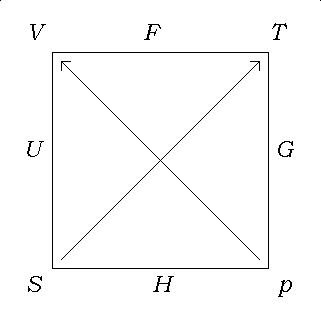
\includegraphics[width=0.5\textwidth]{potenciales}
\caption{Regla mnemotécnica para los potenciales termodinámicos}
\label{fig:potenciales}
\end{figure}

\subsection{Funciones de Massieu}
Las funciones de Massieu son las transformada de Legendre de la entropía, que podemos llamar entropías libres.
La primera es el potencial de Massieu
\begin{equation}
\begin{gathered}
\Phi = S[T,V,\{X_i\}] = S - \frac{U}{T}\\
d\Phi = -U d\frac{1}{T} + \frac{p}{T} dV + \frac{Y_i}{T} dX_i\\
d\Phi = \frac{U}{T^2} dT + \frac{p}{T} dV + \frac{Y_i}{T} dX_i
\end{gathered}
\end{equation}
Ese potencial lo podemos entender como
\begin{equation}
\Phi = - \frac{F}{T}
\end{equation}
Lo mismo podemos hacer con la energía libre de Gibbs, llamada entropía libre de Gibbs o potencial de Planck,
\begin{equation}
\begin{gathered}
\Xi = S[T,p,\{X_i\}] = S - \frac{U}{T} - \frac{p}{T} V = - \frac{G}{T} = \Phi - \frac{p}{T} V\\
d\Xi = -U d\frac{1}{T} - V d\frac{p}{T} + \frac{Y_i}{T} dX_i\\
d\Xi = \frac{U + p V}{T^2} dT - \frac{V}{T} dp + \frac{Y_i}{T} dY_i
\end{gathered}
\end{equation}
Estas funciones son útiles en mecánica estadística, ya que el logaritmo de la función de partición (por la constante de Boltzmann) es igual a la función de Massieu respectiva a la condición del sistema.

\section{Relaciones fundamentales}

\subsection{Relaciones de Maxwell}
Para cualquier función $f(x,y)$ con diferencial
\[df = \frac{\partial f}{\partial x} dx + \frac{\partial f}{\partial y} dy\]
se verifica que 
\[\frac{\partial^2 f}{\partial x y} = \frac{\partial^2 f}{\partial y x}\]
si el diferencial es exacto, es decir si
\[\oint df = 0\]

Podemos encontrar una relación por cada función de estado, que llamamos \emph{relaciones de Maxwell}.

\subsection{Relaciones materiales}

\begin{equation}
C = \frac{\delta Q}{d T} = T \frac{dS}{dT}
\end{equation}

\begin{equation}
C_v = \left.\frac{\partial U}{\partial T}\right|_V = T \left.\frac{\partial S}{\partial T}\right|_V
\label{eq:cv}
\end{equation}

\[C_p = T \frac{dS}{dT} = T \frac{\partial S}{\partial T} + T \frac{\partial S}{\partial V} \frac{dV}{dT} = C_v + T \left.\frac{\partial S}{\partial V}\right|_T \left.\frac{\partial V}{\partial T}\right|_p\]

\[\left.\frac{\partial S}{\partial V}\right|_T = \left.\frac{\partial p}{\partial T}\right|_V\]
con lo que obtenemos
\[C_p = C_v + T \left.\frac{\partial p}{\partial T}\right|_V \left.\frac{\partial V}{\partial T}\right|_p = C_v + T V \alpha \left.\frac{\partial p}{\partial T}\right|_V\]
Ahí definimos el coeficiente de \emph{expansión térmica} como
\begin{equation}
\alpha = \frac{1}{V} \left.\frac{\partial V}{\partial T}\right|_p
\end{equation}
Para el último término usamos que $dV = 0$, ya que la derivada es a volumen constante, y de la expresión del diferencial $dV$ despejamos $\dfrac{dp}{dT}$, que es
\[ \left.\frac{\partial p}{\partial T}\right|_V = \frac{\partial_T V |_p}{\partial_p V|_T} = \frac{\alpha}{\beta_T}\]
donde se definió la \emph{compresibilidad isotérmica}
\begin{equation}
\beta_T = - \frac{1}{V} \left.\frac{\partial V}{\partial p}\right|_T
\end{equation}
con lo que finalmente nos queda
\begin{equation}
C_p = C_v + T V \frac{\alpha^2}{\beta_T}
\end{equation}

Si tenemos tres de las relaciones materiales podemos deducir las demás.

Y podemos a su vez conseguir una relación entre la compresibilidad isotérmica y la \emph{compresibilidad isoentrópica}
\begin{equation}
\beta_S = - \frac{1}{V} \left. \frac{\partial V}{\partial p}\right|_S
\end{equation}
que es
\begin{equation}
\beta_T = \beta_S + \frac{T V \alpha^2}{C_p}
\end{equation}

\subsection{Ecuaciones características}
Experiencia o mecánica estadística $\implies$ potencial termodinámico en variables naturales, llamado \emph{ecuación característica}.

Por ejemplo si tenemos la función $F(T,V,\{X_i\})$ en sus variables, podemos encontrar
\begin{equation}
\begin{gathered}
p = - \left.\frac{\partial F}{\partial V}\right|_{T}\\
S = - \left.\frac{\partial F}{\partial T}\right|_{V}\\
\end{gathered}
\end{equation}
y las relaciones de Maxwell acordes
\begin{equation}
\left.\frac{\partial p}{\partial T}\right|_V = \left.\frac{\partial S}{\partial V}\right|_T
\end{equation}
Además sabemos que $U = F + TS$, se tiene
\begin{equation}
C_v = \left.\frac{\partial U}{\partial T}\right|_V = T \left.\frac{\partial^2 F}{\partial T^2}\right|_V
\end{equation}

Lo mismo podemos hacer para los demás potenciales
\begin{equation}
\begin{gathered}
    S = - \left.\frac{\partial G}{\partial T}\right|_p\\
    V = \left.\frac{\partial G}{\partial p}\right|_T\\
    \frac{\partial S}{\partial V} = \frac{\partial V}{\partial T}\\
    C_p = -T \frac{\partial^2 G}{\partial T^2}\\
    \beta_T = - \frac{1}{V} \frac{\partial^2 G}{\partial p^2}
\end{gathered}
\end{equation}

\begin{equation}
\begin{gathered}
    T = \left.\frac{\partial H}{\partial T}\right|_p\\
    V = \left.\frac{\partial H}{\partial p}\right|_T\\
    \left.\frac{\partial V}{\partial S}\right|_p = \left.\frac{\partial T}{\partial p}\right|_S\\
    \beta_S = - \frac{1}{V} \frac{\partial^2 H}{\partial p^2}
\end{gathered}
\end{equation}

\subsection{Ecuaciones de estado}
Una ecuación de estado se llama a una relación
\begin{equation}
Y_i = Y_i(\{X_j\})
\end{equation}
es decir una variable intensiva en función de las extensivas.
Ejemplos de eso puede ser
\[p = p(U,V) = p(S,V)\]
\[T = T(S,V) = T(U,V)\]
En general para gases tenemos que
\[p = p(T,V,N)\]
donde eliminamos $S$ por $T$ usando una transformación de Legendre.

Tener una ecuación de estado no te da toda la información termodinámica, pero teniendo todas las posibles para un sistema es equivalente a tener una ecuación característica, o tener las tres propiedades materiales necesarias por fase.

$r$ componentes $\implies r + 2$ ecuaciones (asumiendo que no hay más parámetros extensivos que $S$, $V$ y $N_i$), pero la relación de Gibbs-Durheim podemos eliminar una ecuación, obteniendo $r + 1$ grados de libertad.

\section{Equilibrio}
$dS = 0 \qquad d^2 S < 0$ para dos sistemas $1$ y $2$, y que $S_T = S_1 + S_2$.

\[\frac{\partial S_1}{\partial X^1_i} dX^1_i + \frac{\partial S_2}{\partial X^2_i} dX^2_i = 0\]

Por lo tanto
\begin{equation}
\frac{\partial S}{\partial X^1_i} = \frac{\partial S}{\partial X^2_i}
\end{equation}
que para substancias definidas por $T$, $p$ y $\mu$ indica que
\begin{equation}
\begin{gathered}
T_1 = T_2 \\
p_1 = p_2 \\
\mu_1 = \mu_2
\end{gathered}
\end{equation}
que son el equilibrio térmico, mecánico y químico respectivamente.

\subsection{Estabilidad}
\[d^2 S \leq 0\]
que implica que la función debe ser concava en un entorno del equilibrio.
Para un máximo el hessiano debe ser definido negativo, y para un mínimo debe ser definido positivo.
El criterio de Sylvester nos indica que una matriz es definida positiva si todos los menores tienen determinantes positivos, o definida positiva si todos los menores con dimensión k pares son negativos y los impares positivos.

En caso de al entropía, que es una función $S(U,V,\{X_i\})$, sabemos que debe ser máxima en el equilibrio, por lo que usando el criterio de Sylvester se llega a que
\begin{equation}
\begin{gathered}
    \left.\frac{\partial^2 S}{\partial U^2}\right|_{V,X_i} \leq 0 \qquad
    \left.\frac{\partial^2 S}{\partial V^2}\right|_{U,X_i} \leq 0\\
    \frac{\partial^2 S}{\partial U^2} \frac{\partial^2 S}{\partial V^2} - \left(\frac{\partial^2 S}{\partial U \partial V}\right)^2 \geq 0
\end{gathered}
\end{equation}

La primera relación la podemos escribir
\[\left.\frac{\partial^2 S}{\partial U^2}\right|_V = - \frac{1}{T^2} \left.\frac{\partial T}{\partial U}\right|_V = - \frac{1}{T^2 C_v} \leq 0\]
lo que nos lleva a
\begin{equation}
    C_v \geq 0
\end{equation}

Para continuar nos conviene ver la energía $U$, que sabemos que debe ser un mínimo, es decir
\begin{equation}
\begin{gathered}
    \frac{\partial^2 U}{\partial S^2} = \left.\frac{\partial T}{\partial S}\right|_V \geq 0 \qquad
    \frac{\partial^2 U}{\partial V^2} = - \left.\frac{\partial P}{\partial V}\right|_S \geq 0\\
    \frac{\partial^2 U}{\partial S^2} \frac{\partial^2 U}{\partial V^2} - \left(\frac{\partial U}{\partial S \partial V}\right)^2 \geq 0
\end{gathered}
\end{equation}

Para los potenciales podemos hacer el mismo proceso, recordando el cambio de signo de la variable que cambiamos, por lo que si para la energía respecto a la entropía es un minimo, el potencial respecto a la temperatura será un máximo.
\begin{equation}
    \left.\frac{\partial^2 F}{\partial^2 T}\right. = \left.\frac{\partial S}{\partial V}\right|_V \leq 0 \qquad
    \left. \frac{\partial^2 F}{\partial^2 V}\right. = \left.\frac{\partial p}{\partial V}\right|_T \geq 0
\end{equation}
\begin{equation}
    \left.\frac{\partial^2 G}{\partial T^2}\right. = \left.\frac{\partial S}{\partial T}\right|_p \leq 0 \qquad
    \left.\frac{\partial^2 G}{\partial p^2}\right. = \left.\frac{\partial V}{\partial p}\right|_T \leq 0
\end{equation}

\begin{equation}
    \left.\frac{\partial^2 H}{\partial S^2}\right. = \left.\frac{\partial T}{\partial S}\right|_p \geq 0 \qquad
    \left.\frac{\partial^2 H}{\partial p^2}\right. = \left.\frac{\partial V}{\partial p}\right|_S \leq 0
\end{equation}
De estas expresiones podemos deducir las condiciones para las propiedades materiales
\begin{equation}
\begin{gathered}
    C_{V,p} \geq 0\\
    \beta_{T,S} \geq 0\\
    \alpha_{P,V} \geq 0
\end{gathered}
\end{equation}
Pero además si consideramos la siguiente idéntidad
\begin{equation}
    \frac{\beta_S}{\beta_T} = \frac{C_V}{C_p}
\end{equation}
encontramos que
\begin{equation}
    \beta_T \geq \beta_S \geq 0 \qquad C_p \geq C_V \geq 0
\end{equation}

\subsection{Principio de Le Chatelier}
Este principio dictamina que cualquier inhomogeneadad de un sistema en equilibrio tenderá al sistema a otro nuevo equilibrio, volviendo a la homogeneidad.
Esto lo podemos deducir sabiendo que las relaciones materiales son positivas.

Pero también podemos deducir que el comportamiento del sistema frente a fluctuaciones de un parámetro intensivo $X^f$ cualquiera.
Para eso, tomemos dos subsistemas $1$ y $2$, tal que el sistema esté aislado.
El cambio del parámetro $Y$ del sistema $1$ va a ser
\[dY^f_2 = \frac{\partial Y_1}{\partial X_1} dX^f_1\]
además que altera al sistema $2$
\[ dY^f_2 = \frac{\partial Y_2}{\partial X_1} dX^f_1\]
Pasemos a describir el cambio de la energía debido a las respuestas.
\[d(U + U^r) = (Y_1 - Y^r_1) dX^r_1 + (Y_2 - Y^r_2) dX^r_2 \leq 0 \]
donde usamos que la energía debe ser un mínimo.
La expresión de arriba puede llevar finalmente a
\[ d(U + U^r) = dY^f_1 dX^r_1 + dY^f_2 dX^r_2 \leq 0\]
Como los diferenciales son independientes, tenemos que
\[dY^f_1 dX^r_1 = \frac{\partial Y_1}{\partial X_1} dX^f_1 dX^r_1 \leq 0\]
\[dY^f_2 dX^r_2 = \frac{\partial Y_2}{\partial X_1} dX^f_1 dX^r_2 \leq 0\]
La primera desigualdad nos indica que
\begin{equation}
dX^f_1 dX^r_1 \leq 0
\end{equation}

La segunda desigualdad la podemos trabajar usando una relación de Maxwell derivada de la energía
\[ \frac{\partial Y_2}{\partial X_1} = \frac{\partial Y_1}{\partial X_2}\]
en la forma
\[dX^f_1 \frac{\partial Y_1}{\partial X^2} dX^r_2 \leq 0.\]
Si multiplicamos a ambos lados por $\partial_{X_1} Y_1$ que sabemos que es positiva obtenemos
\[\frac{\partial Y_1}{\partial X_1} dX^f_1 \frac{\partial Y_1}{\partial X_2} dX^r_2 \leq 0\]
que es lo mismo que
\begin{equation}
dY^f_1 dY^r_1 \leq 0
\end{equation}
Nuevamente encontramos que la fluctuación del parámetro intensivo genera una respuesta contraria, en línea con el principio de Le Chatelieur.

\section{Cambio de fases}
Toda transición de fase está caracterizada por una perdida de estabilidad de la substancia analizada en el sistema.
\begin{itemize}
\item Primer orden: calor latente, descontinuidad en primeras derivadas. Minimos de potencial separados por una barrera de energía.
\item Segundo orden: continuas, desigualdades en derivadas superiores (segundas y más). Suceden en el mismo estado.
\end{itemize}

El calor latente
\begin{equation}
l = T \Delta s
\end{equation}
siendo $\Delta s$ la diferencia de entropía molar entre las fases.

Como estamos hablando de una transiciones que ocurren a temperatura constante (y las fluctuaciones son debidas a alguna otra variable), trabajaremos con las energías libres.
En esas energías libres se observa la existencia de dos mínimos, uno más estable que otro (a menor energía libre, más estable).
Como la transición se efectúa a temperatura constante, debe haber un cambio de entropía (que lo tratamos de forma molar, para eliminarnos la cantidad de materia).
\subsection{Coexistencia de fases}
Usamos que es un equilibrio entre dos especie
\[\mu_{1} = \mu_{2}\]

Trataremos coexistencia de fases con presión y temperatura, ya que los casos que nos preocupan hay variaciones importantes de volumen molar.
Elijamos dos estados $A$ y $A'$ sobre la curva de coexistencia, pero de diferentes fases, lo mismo con $B$ y $B'$.
La diferencia de presión entre $A$ y $B$ la consideramos
\[p_B - p_A = dP\]
y lo mismo para la temperatura
\[T_B - T_A = dT\]
La curva de coexistencia tiene de pendiente $dp/dT$ en un diagrama $p-T$
Como estoy en un equilibrio de fases
\[\mu_A = \mu_A' \qquad \mu_B = \mu_B'\]
por lo que
\[\mu_B - \mu_A = \mu_B' - \mu_A'\]
y usando que $\mu$ es la energía libre por mol
\[\mu_B - \mu_A = -s dT + v dp = \mu_B' - \mu_A' = -s' dT + v' dp\]
de lo que deducimos finalmente
\begin{equation}
    \frac{dp}{dT} = \frac{s' - s}{v' - v} = \frac{\Delta s}{\Delta v} = \frac{l}{T \Delta v}
    \label{eq:clausius_clayperon}
\end{equation}
Esta es la ecuación de Clayperon, que determina la pendiente de las curvas de coexistencia, y además tiene embuido el principio de Le Chatelieur.
\[d\mu = \frac{V} dp + S dT\]

\subsection{Isotermas inestables}

A saber, la segunda ley determina que
\[ \frac{\partial p}{\partial V}_T \leq 0\]
que en algunas ecuaciones de estado para gases no se cumple.
Esto ocurre debido a que la ecuación de estado está derivada de ciertas hipótesis mecánicas sobre la substacia, pero que algunas de las hipótesis se violan en la inestabilidad.

Como estamos en un cambio de fases, debemos considerar el potencial químico entre dos estados sobre la isoterma, el cual podemos calcular por medio de la relación de Gibbs Durheim
\begin{equation}
    \mu_B - \mu_A = \int^B_A v dP
    \label{eq:isoterma_eq_fase}
\end{equation}
donde la constante de integración dependiente de la temperatura se eliminó al calcular variaciones del potencial químico.
Definido el potencial químico, la energía libre de Gibbs molar, y sabiendo que la presión en función del volumen tiene derivada positiva en algún intervalo, podemos deducir que el volumen respecto a la presión va a ser una función multivaluada.
De esta forma al integrar el volumen, la energía libre también será multivaluada, llevando a una contradicción.
Para salvar la contradicción, exigimos que el potencial químico en todo ese intervalo sea constante, propio de una curva de coexistencia de fases, por lo que la integral de \ref{eq:isoterma_eq_fase} esa nula
\begin{equation}
    \int^B_A v dp = 0
    \label{eq:regla_maxwell}
\end{equation}
que se llama regla de Maxwell, que para una isoterma oscilante exige areas iguales.

Para un gas de Van der Walls la forma de la curva de coexistencia será una recta horizontal generando areas iguales.
Recién cuando truncamos la isoterma con la regla de Maxwell tenemos una curva físicamente posible.
Esa curva crea un cambio brusco de $v(p)$, del volumen molar, por lo que también produce un cambio brusco de la entropía molar.
Como la entropía es una función de estado podemos integrarla con
\[ \Delta s = \int \left.\frac{\partial s}{\partial v}\right|_T dv = \int \left.\frac{\partial p}{\partial T}\right|_V dv\]
sobre la curva ficticia.

El cambio de entropía corresponde a un calor latente intercambiado.
Esto conlleva también un cambio de la energía interna molar, ya que
\[ \Delta u = T \Delta s - p \Delta v\]

Si unimos los extremos de las rectas de coexistencia según la regla de Maxwell obtenemos una curva tipo parabóla, que separa el diagrama $p-v$ en dos fases, gaseosa y líquido más gas.

La fracción de gas y líquido en la zona de coexistencia viene dado por la regla de la palanca, que corresponde a asumir que existe una sóla substancia con volumen $V = N v$, divida en dos subsistemas con volumenes $V_G = N x_g v_G$ y $V_L = N x_L v_L$, siendo $x_i$ la fracción molar ($\sum x_i = 1$).
Finalmente la regla queda
\begin{equation}
x_L = \frac{v_G - v}{v_g - v_L} = 1 - x_G
\end{equation}

La inestabilidad de un potencial genérico en función de sus variables $X_j$ lo podemos corregir uniendo con una línea recta los dos mínimos separados por una barrera, como vemos en la figura \ref{fig:fase_potencial}
\begin{figure}[H]
\centering
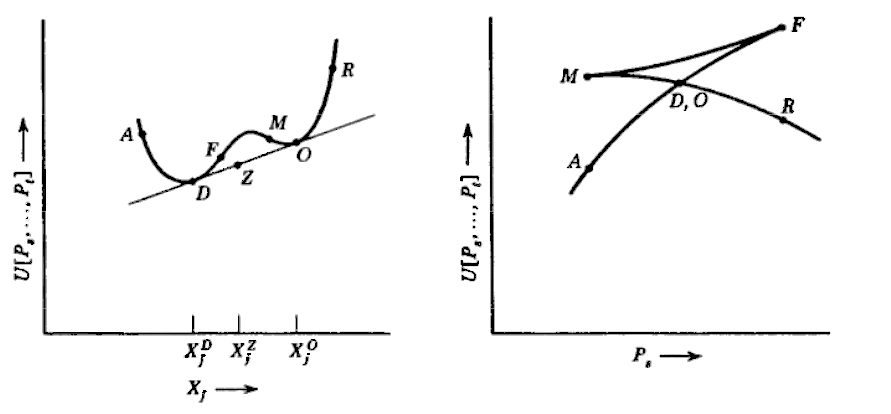
\includegraphics[width=0.5\textwidth]{fase_potencial}
\caption{Potencial generalizado en un caso de perdida de estabilidad, además de la correción con el método de Maxwell}
\label{fig:fase_potencial}
\end{figure}


\subsection{Regla de las fases de Gibbs}

\begin{equation}
f = 2 + M(r - 1) - r(M - 1) = r - M + 2
\label{eq:regla_gibbs_fase}
\end{equation}


\section{Tercer principio}

\begin{law}[Mínimo de la entropía]
La entropía de un sistema tiende a una constante positiva al hacer nula la temperatura. Es decir
\[\displaystyle\lim_{T \to 0} S = S_0 \geq 0\]
Este valor corresponde al mínimo de entropía.
\end{law}
De esta ley, junto con la segunda ley, podemos deducir que no es posible alcanzar la temperatura $T = 0$ llamado cero absoluto.


\section{Gases reales e ideales}

\subsection{Gas ideal}

\begin{equation}
p V = n R T
\label{eq:gas_ideal_estado}
\end{equation}


\begin{figure}[H]
\centering
%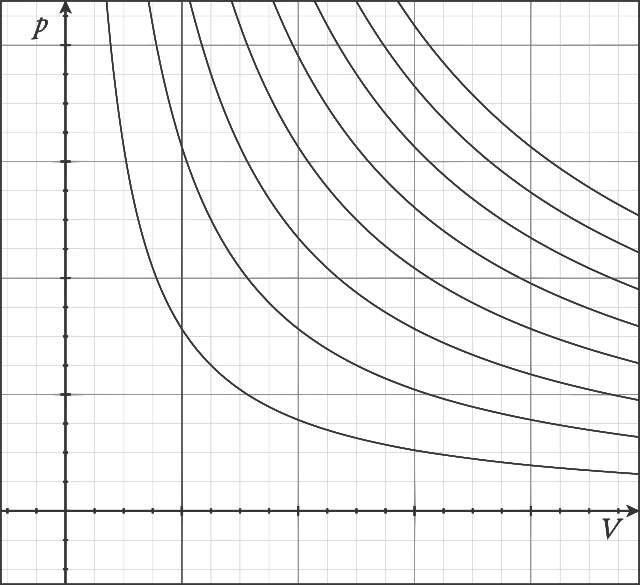
\includegraphics[width=0.4\textwidth]{gas_ideal_isotermas}
\caption{Isotermas de un gas ideal con unidades arbitrarias}
\label{fig:gas_ideal_isotermas}
\end{figure}

La energía $U$ no depende del volumen, ya que si tomamos el diferencial de entroía
\[ dS = \left.\frac{\partial S}{\partial T}\right|_V dT + \left.\frac{\partial U}{\partial V}\right|_T dV\]
y lo reemplazo en la expresión de la primera/segunda ley
\[ dU = T \left.\frac{\partial S}{\partial T}\right|_V dT + \left( T \left.\frac{\partial S}{\partial V}\right|_T - p \right) = C_v dT + \left( T \left.\frac{\partial p}{\partial T}\right|_V - p \right) = C_v dT \]

\begin{equation}
    dU = C_v dT
    \label{eq:gas_ideal_energia}
\end{equation}
Experimentalmente (y de la mecánica estadística) se encuentra que el calor específico es constante con la temperatura y que además vale
\begin{equation}
    C_v = \frac{3}{2} N k_B
    \label{eq:gas_ideal_cv}
\end{equation}

Ergo
\begin{equation}
    U = \frac{3}{2} N k_B T
\end{equation}
donde aparece la \emph{equipartición de la energía} en forma de tres grados de libertad con $\frac{N k_B T}{2}$ energía, y también podemos encontrar la entropía
\begin{equation}
    S = C_v \ln\left(\frac{T}{T_0}\right) + N K \ln\left(\frac{V}{V_0}\right)
\end{equation}

A partir de la expresión de la entropía podemos deducir la funciona de una transformación adiabática, usando que la entropía $S = cte$,
\begin{equation}
    V T^{\frac{C_v}{N k_B}} = c \qquad T V^{\frac{N k_B}{C_v}} = c
\end{equation}
que se puede llevar a
\begin{equation}
    p V^{1 + \frac{C_v}{N k_B}} = p V^{\frac{C_v + N k_B}{C_v}} = p V^{\gamma} = c
    \label{eq:gas_ideal_adiabaticas}
\end{equation}

Tenemos además
\begin{equation}
    C_p - C_v = N k_B
\end{equation}
por lo que
\begin{equation}
    \gamma = \frac{C_p}{C_v}
\end{equation}
que para un gas ideal monoatómico es igual a $\gamma \dfrac{3}{2}$.

\subsection{Gas de Van der Waals}

\begin{equation}
    \left(p + \frac{a N^2}{V^2}\right)(V- b N) = N k_B T
    \label{eq:vanderwalls}
\end{equation}
que podemos escribir de la siguiente forma
\begin{equation}
    p = \frac{R T}{v - b} - \frac{a}{v^2}
    \label{eq:vanderwalls_intensivo}
\end{equation}

Veamos las isotermas, que las graficamos en la figura \ref{fig:gases_vdw_isotermas}
\begin{figure}[H]
    \centering
    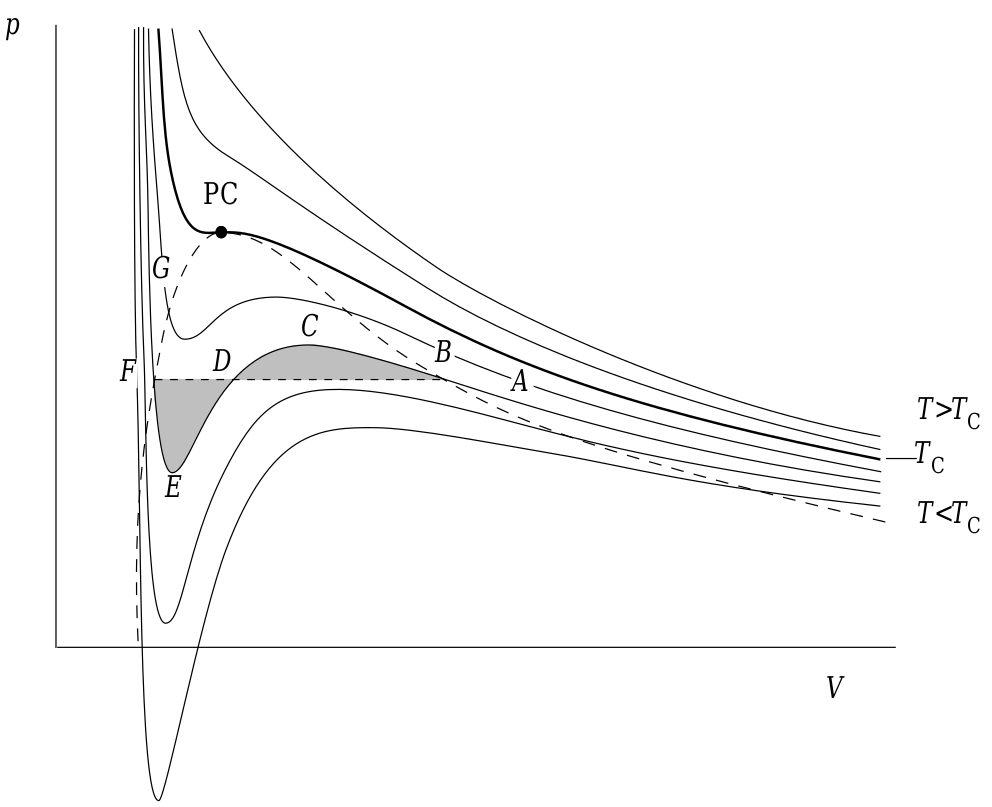
\includegraphics[width=0.5\textwidth]{gases_vdw_isotermas}
    \caption{Diagrama p-V con isotermas, adimensionalizadas, del gase de Van der Waals, más el punto crítico y la zona de coexistencia}
    \label{fig:gases_vdw_isotermas}
\end{figure}


En el punto crítico tenemos que
\begin{equation}
    \left.\frac{\partial p}{\partial V}\right|_{T_c} = 0 \qquad \left.\frac{\partial^2 p}{\partial V^2}\right|_{T_c} = 0
\end{equation}
La primer condición y la segunda condición implican que
\begin{equation}
    v^3 = \frac{2 a}{k_B T_c} (v - b)^2 \qquad 3 v^2 = \frac{4 a}{k_B T_c} (v - b)
\end{equation}

Dividimos una por otra y obtenemos que
\[ \frac{1}{2} v = \frac{1}{2} (v - b) \]
lo que es lo mismo que el volumen crítico es igual
\begin{equation}
    v_c = 3 b
\end{equation}
Ahora despejamos la temperatura crítica por la constante de Boltzmann de la derivada segunda tenemos
\begin{equation}
    k_B T_C = \frac{8}{27} \frac{a}{b}
\end{equation}
De esta forma reemplazando la temperatura crítica y el volumen crítico en la ecuación de Van der Waals tengo la presión crítica
\begin{equation}
p_C = \frac{k_B T_C}{v_C - b} - \frac{a}{v^2_C} = \frac{1}{9} \frac{a}{b^2} \left(\frac{4}{3} - 1\right)
\end{equation}
Ahora si elijo variables $v = v' v_c$, $p = p' p_c$ y $T = t' T_c$ y las reemplazo en la ecuación de Van der Waals
\[ \left(p' p_c + \frac{a}{v'^2 v^2_c}\right) (v' v - b) = k_B T t' \]
que termina resultando en
\begin{equation}
\left(p' + \frac{3}{v'^2}\right)(3 v' - 1) = 8 t'
\label{eq:gases_estados_correspondientes}
\end{equation}
que es una relación independiente de la substancia llamada ley de los estados correspondiente, 

\subsection{Ecuación del Virial}

\begin{equation}
p v = RT \left( 1 + \sum_{i = 1} \frac{A_i}{v^i}\right)
\end{equation}
con cada coeficiente función solamente de la temperatura, y representa aspectos de las interacciones entre moléculas.
Esa expresión se denomina ecuación del estado virial.

%\section{Introducción a la mecánica estadística}


\chapter{Mecánica cuántica}

\section{Desarrollos históricos}

\subsection{Teoría atómica}
La naturaleza atómica y \emph{cuantizada} de la materia no se aceptó hasta empezado el siglo XX, cuando teorías como el movimiento browniano (explicado por Einstein en 1905) basados en la teoría cinética (propuesta por Joule y Boltzmann en 1860) lograron explicar muchisimas experiencias y además eran consistentes con los experimentos.

Modelos históricos (ordenados en tiempo y sin contar el modelo de Demócrito)
\begin{itemize}
\item Modelo de Thompson: Budin de pan, con pasa iguales a los electrones. Explica existencia de carga negativa y la radiación de los espectros.
\item Modelo de Rutherform: Modelo planterario, explica la dispersión de particulas, pero no explica la inestabilidad.
\item Modelo de Bohr: cuantización de orbitas $L = n\hbar$, orbitas no permitidas. $h \nu = \Delta E$. Explicación de Sommerfeld-Wilson $\displaystyle \oint p dq = n h$
\end{itemize}

\subsection{Cuerpo negro}
La radiación de cuerpo negro consiste en un cuerpo en equilibrio térmico con la radiación, con el énfasis en la forma de la radiación.
Para eso sabemos de la mecánica estadística que la presión de radiación es
\[ p = \frac{u}{3} \]
donde $u$ es la densidad de energía. 
\[dU = d(u V) = V du + u dV = T dS - p dV = T d(s V) - \frac{u}{3} dV = T s dV + T V ds - \frac{u}{3} dV\]
y si usamos que $u(T)$ y $s(T)$, ya que no hay otra variable termodinámica, llegamos a
\[ \left( \frac{\mathrm{d} u}{\mathrm{d} T} - T \frac{\mathrm{d} s}{\mathrm{d} T} \right) dT = \left(s T - \frac{4}{3} u \right) \frac{dV}{V}.\]
Ergo
\begin{equation}
\begin{gathered}
 s = \frac{4}{3} \sigma T^3\\
 u = \sigma T^4
\end{gathered}
\end{equation}
que corresponde a la ley de Stefan-Boltzmann, con la constante 
\begin{equation}
\sigma = 5,67\times 10^{-8} \rm\textstyle \frac{W}{m^2 \cdot K^4} 
\end{equation}

Pensemos en una caja en equilibrio térmico, por lo que hay ondas estacionarias, y consideremos la integral de cada onda plana con condiciones de contorno adecuadas.
Eso representa la energía por unidad de volumen
\begin{equation}
 u = \frac{1}{\pi^2 c^3} \int^\infty_0 \nu^2 f(\nu,T) d\nu
\end{equation}
Nos queda saber la forma de la función de $f(\nu,T)$.

\begin{itemize}
    \item{Ley de Wien}
    \item{Rayleigh-Jeans: modelo ondulatorio clásico}
\end{itemize}

Para eso Planck propone el siguiente desarrollo, usando la la mecánica estadística: 
como estamos en equilibrio térmico, la probabilidad de encontrar el sistema con energía $\varepsilon$ es 
\[ P(\varepsilon) = e^{-\beta \varepsilon}\]
con lo que el valor medio de la energía va a ser
\[ \langle E \rangle = \frac{\int \varepsilon e^{-\beta \varepsilon} d\varepsilon}{\int e^{-\beta \varepsilon'} d\varepsilon'} = \frac{1}{Z} \int \varepsilon e^{-\beta \varepsilon} d\varepsilon\]
A partir de acá, Planck propone que la energía de cada oscilador es un múltiplo de $h\nu$, constante que denominó con su nombre, con valor (actual) de
\begin{equation}
h = 6,626 \times 10^{-27}\,\text{erg}\,\text{s}.
\end{equation}
Sabiendo que la energía de cada oscilador estaba \emph{cuantizada} o discretizada, la función de partición pasa a ser
\[ Z = \sum^\infty_{n = 0} e^{-n \beta \varepsilon} = \frac{1}{1 - e^{-\beta \varepsilon}}\]

De la mecánica estadística tenemos
\begin{equation}
    \langle E \rangle = - \frac{\partial}{\partial \beta} \ln(Z)
\end{equation}
por lo que finalmente nos queda que que la densidad de energía con la proposición de Planck es
\begin{equation}
  u = \frac{1}{\pi^2 c^3} \int^\infty_0 \frac{h \nu^3}{e^{\beta h \nu} - 1} d\nu
\end{equation}
que se llama ley de Planck.

Si resolvemos la integral, llegamos a la ley  de Stefan-Boltzmann, con la constante igual 
\begin{equation}
\sigma=\frac{2\pi^5 k^4}{15c^2h^3}= 5.6704 \cdot 10^{-8}\; \rm\frac {W}{m^2 \cdot K^4}
\end{equation}

\subsection{Efecto fotoeléctrico}

El efecto fotoeléctrico se observa a tener un tubo con dos electrodos, ánodo y cátodo, y el aire enrarecido o vació. Al iluminar el cátodo se logra mejorar la descarga de electrones, observada en un aumento en la corriente entre ánodo y cátodo.

La intensidad de la luz sólo determina la corriente máxima o de saturación, y el material y la longitud de onda incidente determina el potencial de frenado.

En 1905, Einstein propone que la naturaleza de la luz debe ser curpurscular, con el cuánto llamado \emph{fotón}, con energía $E = h \nu$.
De esa forma la energía cinética que tendrá un fotón es
\begin{equation}
    K = h \nu - \phi
\end{equation}
donde $\phi$ es el trabajo necesario para sacar un electrón del metal.
Defino la función trabajo $\phi_0$ tal que
\begin{equation}
  K_{max} = h\nu - \phi_0
\end{equation}

Finalmente podemos obtener el potencial de frenado sabiendo que la energía cinética máxima es igual a $eV_0$, de electromagnetismo clásico, es decir
\begin{equation}
 V_0 = \frac{h}{e} \nu - \frac{\phi_0}{e}
 \label{eq:fotoelectrico}
\end{equation}


\subsection{Efecto Compton}
Dispersión producto de interacción radiación materia, de media energía. 
En general se observa con radiación X o gamma de baja frecuencia.

Aún con una fuente monocromática incidente, el haz de luz dispersado un ángulo $\theta$ tiene dos longitudes de onda, $\lambda$, la original, $\lambda'$, tal que  $\Delta \lambda = \lambda' - \lambda$ es una magnitud positiva.
La diferencia se denomina corrimiento Compton, y experimentalmente se observa que depende del ángulo y no del material.

Para explicarlo Compton propuso que la luz incidente está compuesta por fotones, y que al incidir sobre los electrones, que los consieraba libres y en reposo (buscando independencia del material), ceden parte de su energía, por lo que $E' < E$ y como la energía de cada fotón es $E = h \nu$, entonces $\lambda' > \lambda$.

Para poder analizar la colisión debemos considerar la conservación del cuadrimomento
\[ p^\mu = (E/c, \textbf{p}) = cte\]
La energía relativista corresponde a
\[ E = \sqrt{(cp)^2 + (m c^2)^2} \]
que al considerar el electrón inicialmente quieto y la masa nula del fotón
\[E + m_e c^2 = E' + m_e c^2 + K \]
\[K = E - E' = c (p - p') \]
Mientras la conservación del momento lineal, en x e y, consiste en
\begin{gather*}
    p = p' \cos(\theta) + p_e \cos(\phi)\\
    0 = p' \sen(\theta) - p_e \sen(\phi)
\end{gather*}
Si eliminamos $\phi$, que es ángulo de dispersión de electrón, obtenemos
\[p^2 + p'^2 - 2 p p' \cos(\theta) = p^2_e \]

Ahora si usamos la energía cinética $K$ en la energía relativista
\[ E_e^2 = (K + m_e c^2)^2 = c^2 p^2 + m^2 c^4\]
que se reduce a
\[ 2 K m_e + \left(\frac{K}{c}\right)^2 = 2 m_e c (p - p') + (p - p')^2 = p_e^2\]

Ahora eliminamos $p_e$ de estas ecuaciones, llegando a
\[m_e c (p - p') = p p' (1 - \cos(\theta)\]
y finalmente se rescribe un poco usando que para los fotones $p = h/\lambda$, obteniendo
\begin{equation}
    \Delta \lambda = \lambda' - \lambda = \frac{h}{m_e c} \left(1-\cos \theta \right)
\end{equation}

\section{Formulación ondulatoria}

De Broglie, propuso la materia también tenga una dualidad onda-partícula.
Para eso de Broglie propone la existencia de ondas pilotos, que determina el movimiento de la partícula, que tienen por longitud de onda y energía relativista (impulsados por la energía del fotón de Einstein)
\begin{equation}
    p = \hbar k = \frac{h}{\lambda} \qquad E = h\nu
\end{equation}

Toda onda unidimensional (para simplificar la notación) se puede pensar como la superposición de ondas planas, con una amplitud y fase para cada una, es decir
\begin{equation}
    \Psi(x,t) = \int_{-\infty}^{\infty} A(k') e^{-i\psi(k')} e^{i (k' x - \omega' t)} dk'
\end{equation}
y sabiendo además que
\[ k' = \frac{p}{\hbar} \qquad \omega' = \frac{E'}{\hbar}\]
Si elegimos a la energía como $E' = m \gamma(v') c^2$ y $p = m \gamma(v') v'$, encontramos que la velocidad de propagación de la onda piloto es
\begin{equation}
    v_f = \frac{\omega'}{k'} = \frac{E'}{p'} = \frac{c^2}{v'}
\end{equation}
Esta velocidad es mayor que la de la luz, pero no debería preocuparnos porque la partícula realmente se mueve a la velocidad de grupo
\begin{equation}
    v_g = \left.\frac{\partial \omega}{\partial k'}\right|_k = \frac{\partial E}{\partial p} = c^2 \frac{p}{E} = v
\end{equation}
donde usamos que $E^2 = c^2 p^2 + m^2 c^4$, $E = \gamma m c^2$ y $p = m v$.

\subsection{Principio de incerterza}
El postulado de ondas pilotos también trae consigo la imposibilidad de observar la posición de la onda y su cantidad de movimiento, ya que una partícula localizada espacialmente tiene amplitud no nula, pero su momento no queda definido con la misma certeza.
Esto imposibilidad en la medición fue propuesta por Heisenberg, y se denomina principio de incerteza. 
El proceso de medir implica alterar el sistema, imposibilitando otras medidas.

La transformada de Fourier de una función $f(r)$ corresponde a
\begin{equation}
    F(s) = \frac{1}{\sqrt{2\pi}} \int_{-\infty}^{\infty} f(r) e^{i r s} \mathrm{d}r
\end{equation}
y la antitransformada o inversa
\begin{equation}
    f(r) = \frac{1}{\sqrt{2\pi}} \int_{\infty}^{\infty} F(s) e^{- i r s} \mathrm{d}s
\end{equation}

si consideramos $s = k = p/\hbar$ y $r = x$, tenemos que
\begin{equation}
    \psi(x, t) = \frac{1}{\sqrt{2 \pi \hbar}} \int_{-\infty}^{\infty} \phi(p, t) e^{i p x/\hbar}\, \mathrm{d}p
\end{equation}

Ahora pidamos un espectro de posiciones o de momento gaussiano, que al tomar la varianza nula se transforma naturalmente en la posición o momento bien definda.
Es decir que tenemos que
\[ \phi(k) \propto e^{-\left(k/2\Delta k\right)^2} \]
La transformada de Fourier de una gaussiana es también una gaussiana
\[ \psi(x) \propto e^{-\left(x/2\Delta x\right)^2}\]
pero de la teoría de Fourier determina que para paquetes guassianos las varianzas tendrán de relación
\begin{equation}
    \Delta x \Delta k = \Delta x \frac{\Delta p}{\hbar} \frac{1}{2}
\end{equation}
y además, para paquetes no gaussianos determina que
\begin{equation}
    \Delta x \Delta k = \Delta x \frac{\Delta p}{\hbar} \leq \frac{1}{2}
\end{equation}
Estas expresiones anteriores determinan el límite inferior para el producto de las incertezas, y por eso determina la precisión que se pueden tener en las mediciones.

\subsection{Ecuación de Schrödinger}
Schrödinger en su ecuación de onda, propuso restringir los postulado de Broglie a la mecánica clásica (aunque estos sean compatibles con la relatividad especial) y además abandonó el concepto de onda piloto y llamó a la función $\psi$ como \emph{función de onda}.

\begin{equation}
    i \hbar \frac{\partial \psi}{\partial t} = - \frac{\hbar}{2m} \frac{\partial^2 \psi}{\partial x^2} + V \psi
\end{equation}
que se puede extrapolar a varias dimensiones fácilmente
\begin{equation}
- \frac{\hbar^2}{2m} \nabla^2 \psi(\textbf{r},t) + V(\textbf{r},t) \psi(\textbf{r},t) = i \hbar \frac{\partial \psi(\textbf{r},t)}{\partial t}
\end{equation}

La función de onda es interpretable como
\begin{equation}
    P(x, t) dx = \frac{|\psi(x, t)|^2 \mathrm{d}x}{\int |\psi(x, t)|^2 \mathrm{d}x} = \frac{1}{Z} |\psi(x, t)|^2 \mathrm{d}x
\end{equation}
donde ya dividimos por la normalización.

El valor medio de cualquier observable $A$ es
\begin{equation}
    \langle A \rangle = \frac{1}{Z} \int A(x, t) \psi \psi * \mathrm{d}x
\end{equation}
por lo que la función de onda tiene toda la información necesaria del sistema, sin representar más que una herramienta matemática.

\subsubsection{Conservación de la probabilidad}
La corriente de probabilidad
\begin{equation}
    \textbf{J}(\textbf{r}, t) = \frac{i \hbar}{2m} \left(\psi \nabla \psi* - \psi* \nabla \psi\right)
    \label{eq:corriente_proba}
\end{equation}
y derivamos la función $\psi \psi*$, obtenemos que
\begin{equation}
    \frac{\partial P}{\partial t} = - \nabla \cdot \textbf{J}
\end{equation}
que equivale a la ecuación de Schrödinger y deja evidente la conservación de la probabilidad (a partir del teorema de Gauss en el infinito).

\subsubsection{Independiente del tiempo}

\begin{equation}
    \psi = \phi(\textbf{r}) e^{i \frac{E}{\hbar} t}
\end{equation}
y la ecuación de Schrödinger es
\begin{equation}
    - \frac{\hbar^2}{2m} \nabla^2 \phi(\textbf{r}) + V(\textbf{r}) \phi(\textbf{r}) = E \phi(\textbf{r})
\end{equation}

\section{Formalismo}

\begin{definition}[Estado]
    El estado del sistema corresponde a su función de onda $\psi(\textbf{r},t)$.
\end{definition}

\begin{definition}[Observable]
    Una magnitud física relevante y medible en un experimento se denominada observable.
\end{definition}

\begin{definition}[Autoestados del observable]
    Los estados que determinan que se mida un observable $A$ y se obtenga una medición $a_i$ con probabilidad 1 se llaman autoestados del observable.
    Los valores $a_i$ se denominan autovalores del observable
    No hay una notación generalizada, nosotros los vamos a llamar $\psi_i$
\end{definition}

\begin{axiom}[Superposición de estados]
    Cualquier estado del sistema es una combinación lineal de autoestados de un observable
    Es decir
    \begin{equation}
        \phi = \sum_k \alpha_k \psi_k \qquad \alpha_k \in \mathbb{C}
    \end{equation}
\end{axiom}

\begin{axiom}[Colapso del estado]
    Si mido el observable y obtengo $a_i$ entonces el estado del sistema está definido en la autoestado asociado (o una combinación de estados asociados) y va a quedar así por siempre.
    Esto se denomina colapso por medición
\end{axiom}

\begin{axiom}[Probabilidad de la medición]
    Si tengo un estado $\psi = \sum_k \alpha_k \psi_k$, combinación lineal de autoestados, la probabilidad de medir de un observable $A$ el valor $a_k$ es $\alpha_k \alpha*_k = |\alpha_k|^2$.
    Esto es una consecuencia \emph{a priori}, que es el poder predictivo que tiene la teoría
\end{axiom}

\subsection{Espacio de estados}

\begin{equation}
    \psi, \phi \in \mathcal{H} \implies \alpha \psi + \phi \in \mathcal{H}, \forall \alpha \in \mathbb{C}
\end{equation}

Con un producto interno
\begin{equation}
    \begin{gathered}
        \phi = \sum_k \alpha_k \phi_k \qquad \psi = \sum_k \beta_k \phi_k \\
        (\phi,\psi) \in \mathbb{C} / (\phi,\psi) = (\psi,\phi)* = \sum_k \alpha*_k \beta_k
    \end{gathered}
\end{equation}

Un espacio $\mathcal{H}$ así se denomina espacio de Hilbert, ya que el producto interno induce una norma.

Los valores medios ahora son
\begin{equation}
    \langle A \rangle = \sum_m \alpha*_m \alpha_m a_m = \sum_m (\phi, \phi_m) (\phi_m, \phi) a_m 
\end{equation}

\subsection{Notación de Dirac}

Los estados los notamos y llamamos ''ket''
\begin{equation}
    |\psi\rangle = \sum_j \alpha_j |j\rangle
\end{equation}

Y asociamos los ''bra'' con el producto interno
\begin{equation}
    \begin{gathered}
    |\psi\rangle = \sum_k \alpha_k |k \rangle \qquad |\phi\rangle = \sum_k \beta_k |k\rangle \\
    \langle \phi | \psi \rangle = \sum_k \beta^*_k \alpha_k \implies \langle \psi | = \sum_k \beta^*_k \langle k|
\end{gathered}
\end{equation}

Como es un producto interno, vale la desigualdad de Cauchy-Schwartz
\begin{equation}
    |\langle \phi | \psi \rangle|^2 \leq (\sum |\beta_j|^2) (\sum |\alpha_j|^2) = 1
\end{equation}

\subsection{Observables y operadores}

\begin{definition}[Operador]
    Un operador es una transformación que toma un estado y devuelve otro estado, no necesariamente en el mismo espacio inicial
    Vamos a notar a los operadores con $\hat{A}$
\end{definition}

Para un observable genérico podemos entonces definir su operador asociado como
\begin{equation}
    \hat{A} = \sum_k a_k |k \rangle\langle k|
\end{equation}
en donde si operamos sobre un ket $|\phi \rangle$
\begin{equation}
    \hat{A} |\phi\rangle = \sum_k a_k |k \rangle \langle k | \phi \rangle = \sum_k a_k |k \rangle \langle k | \left(\sum_j \beta_j |j \rangle\right) = \sum_k a_k \beta_k |k \rangle
\end{equation}
donde usamos la ortogonalidad de la base donde estoy trabajando.
Mientras, si el operador lo aplico a un bra obtengo
\begin{equation}
    \langle \phi | \hat{A} = \left(\sum_j \beta^{*}_j \langle j |\right) \sum_k a_k | k \rangle \langle k | = \sum_k \beta^{*}_k a_k \langle k |
\end{equation}

Acá puedo definir al operador adjunto $A^\dagger$ como el operador que verifica que
\begin{equation}
    (A |\psi \rangle)^\dagger = \langle \psi | A^\dagger
\end{equation}
Un operador tal que $A^\dagger = A$ es un operador autoadjunto, que podemos demostrar que tiene todos sus autovalores reales.

Volviendo, si junto ambas tengo que
\begin{equation}
    \langle \phi | \hat{A} | \phi \rangle = \sum_k \beta*_k \beta_k a_k = \sum_k P(a_k) a_k = \langle A \rangle
\end{equation}
que corresponde al valor medio usual.

Otra propiedad intersante de los operadores es que dada una base de autoestados podemos definir una matriz asociada al operador $\hat{A}$, tal que
\begin{equation}
    (\hat{A})_{n,m} = \langle n | \hat{A} | m \rangle
\end{equation}

\subsection{Incerteza}
Ahora imaginemos que tenemos dos operadores $\hat{A}$ y $\hat{B}$, y dos estados $|\phi\rangle$ y $|\psi\rangle$ tal que
\[ |\phi\rangle = (\hat{A} + i \lambda \hat{B}) |\psi\rangle\]
con $\lambda \in \mathbb{R}$.

La norma del estado $|\phi\rangle$, que no puede ser nula y es real, vale
\[ \langle \phi | \phi \rangle = \langle \psi | (\hat{A} - i \lambda \hat{B}) (\hat{A} + i \lambda \hat{B})|\psi\langle \leq 0\]
si desarrollo los términos
\[ \lambda^2 \langle \psi | \hat{B}^2 |\psi \rangle + \lambda i \langle \psi | [\hat{A},\hat{B}] |\psi \rangle + \langle \psi | \hat{A}^2 | \psi \langle \leq 0 \]
donde definimos al \emph{conmutador} como
\begin{equation}
    [\hat{A},\hat{B}] = \hat{A}\,\hat{B} - \hat{B}\,\hat{A}
  \label{eq:conmutador}
\end{equation}

Llegamos a que la raiz de la cuadrática tiene que ser una o ninguna
\[ 4 a c \leq b^2 \]
que se termina desarrollando en
\begin{equation}
    \langle \hat{A}^2 \rangle \langle \hat{B}^2 \rangle \leq \left(\frac{i}{2} \langle [\hat{A},\hat{B}] \right)^2
\end{equation}
Y si definimos el operador varianza como
\begin{equation}
    \Delta \hat{A} = \hat{A} - \langle \hat{A} \rangle \hat{Id}
\end{equation}
y el cuadrado de la varianza como
\begin{equation}
    (\Delta \hat{A})^2 = \hat{A}^2 - \langle \hat{A}^2 \rangle \hat{Id}
\end{equation}
llegamos a 
\begin{equation}
  \langle(\Delta A)^2\rangle \langle(\Delta B)^2\rangle \geq \frac{1}{4} \langle [A, B] \rangle
\end{equation}

\subsection{Función de onda}

\begin{equation}
    |\psi \rangle = \int |x \rangle \langle x | \psi \rangle \mathrm{d}x
\end{equation}
por lo tanto
\begin{equation}
  \langle x|\psi\rangle = \psi(x) 
\end{equation}
ya que al calcular el valor medio del observable $\hat{x}$ (que representa a la posición) tenemos que
\begin{equation}
    \langle \hat{x} \rangle = \langle \psi | \left( \int |x \rangle x \langle x | \mathrm{d}x \right) | \psi \rangle = \int \langle \psi | x \rangle x \langle x | \psi \rangle \mathrm{d} x = \int x \psi(x) \psi^*(x) \mathrm{d}x
\end{equation}

El operador $\hat{x}$ mientras tiene como autovalores a la posición asociada $x$, es decir
\begin{equation}
    \hat{x} |\psi\rangle = x |\psi\rangle
\end{equation}
De esa forma podemos definir al operador $\hat{x}$ como 
\begin{equation}
\hat{x} = \int |x\rangle x \langle x | \mathrm{d}x
\label{eq:operador_x}
\end{equation}

Puedo hacer el mismo artilugio para el momento lineal, definiendo un operador $\hat{p}$ con autoestados $|p\rangle$ y autovalores $p$.
\begin{equation}
\begin{gathered}
\hat{p} = \int |p\rangle p \langle p | \mathrm{d}p\\
\hat{p} |p'\rangle = p' |p'\rangle
\end{gathered}
\end{equation}
Como sabemos la función de onda asociada a una partícula con el momento definido es una onda plana
\begin{equation}
\langle x | p \rangle = C e^{i \frac{p}{\hbar} x}
\end{equation}

Tenemos la siguiente operación
\[ \langle x' | x \rangle = \delta(x - x')\]
que es lo mismo que
\[ \langle x' | \hat{Id} | x \rangle = \delta(x - x').\]
Ahora si escribimos el operador identidad en alguna base interesante, como se la de momentos, podemos encontrar una expresión para la delta de Dirac
\[ \langle x' |\left( \int |p\rangle \langle p | \mathrm{d}p \right)| x \rangle = \delta(x' - x)\]
\[ \int \langle x' | p \rangle \rangle p | x \rangle \mathrm{d}p = \delta(x' - x)\]
que finalmente nos da
\[ \delta(x' - x) = \int |C|^2 e^{i \frac{p}{\hbar}(x' - x)} \mathrm{d}p\]
Si elijo la constante usando la convención de la transformada de Fourier que usamos
\begin{equation}
 \delta(x' - x) = \frac{1}{2\pi\hbar} \int e^{i \frac{p}{\hbar} (x' - x)} \mathrm{d}p
\end{equation}

Ahora nos queda preguntarnos que produce el operador $\hat{p}$ en un estado arbitrario.
\[ \hat{p}|\psi\rangle = \int |p\rangle p \langle p|\left(\int | x \rangle \langle x |\psi \rangle \mathrm{d}x \right) \mathrm{d}p \]
y si multiplicamos por un bra de posición $\langle x'|$
\[ \langle x' | \hat{p} | \psi \rangle = \iint \langle x'|p\rangle p \langle p | x \rangle \langle x | \psi \rangle \mathrm{d}x\mathrm{d}p = \iint \frac{p}{\sqrt{2\pi\hbar}} e^{i \frac{p}{\hbar} (x' - x)} \psi(x) \mathrm{d}x \mathrm{d}p = -i \hbar \frac{\partial}{\partial x'} \left(\iint \frac{1}{\sqrt{2\pi\hbar}} e^{i \frac{p}{\hbar} (x' - x)} \psi(x) \mathrm{d}p \mathrm{d}x \right)\]
que nos queda finalmente como
\begin{equation}
\langle x | \hat{p} | \psi \rangle = - i \hbar \frac{\partial}{\partial x} \langle x | \psi\langle
\label{eq:operador_p_estado}
\end{equation}
que también lo podemos ver como
\begin{equation}
 \hat{p} \psi(x) = - i \hbar \frac{\partial}{\partial x} \psi(x)
\end{equation}

Algo muy interesante es el conmutador del operador $\hat{x}$ y el operador $\hat{p}$ aplicado a una función de onda cualquiera
\[[\hat{x},\hat{p}]\psi = \hat{x}\hat{p}\psi - \hat{p}\hat{x}\psi = -i \hbar x \frac{\partial \psi}{\partial x} + i \hbar \frac{\partial (x \psi)}{\partial x} = i \hbar \psi \]
es decir 
\begin{equation}
[\hat{x},\hat{p}] = i \hbar \hat{Id}
\end{equation}
propiedad que se denomina relación de conmutación canónica. 
La relación de conmutación canónica nos permite decidir que
\begin{equation}
\Delta p \Delta x \geq \frac{\hbar}{2}
\end{equation}
que corresponde al principio de incerteza de Heisenberg en su formulación original.

\section{Dinámica}

La ecuación de Schrödinger la podemos escribir como
\begin{equation}
  \hat{H} |\psi\rangle = i \hbar \frac{\partial}{\partial t} |\psi\rangle
\end{equation}
si identificamos al operador $\hat{H}$ con el hamiltoneano clásico, y lo llamamos operador hamiltoneano
\begin{equation}
\hat{H} = \frac{\hat{p}^2}{2m} + V(x, t)
\end{equation}
De esta forma el proceso de ''cuantizar'' un sistema de mecánica clásica consiste en escribir el hamiltoneano de dicho sistema con operadores y posteriormente resolver la ecuación diferencial asociada.

En el caso que no dependa del tiempo el potencial la ecuación queda, con el operador hamiltoneano
\begin{equation}
\hat{H} |\psi \rangle = E | \psi \rangle
\end{equation}

\subsection{Potencial nulo}
Si el potencial es nulo $V = 0$ y estamos en el caso unidimensional, entonces debemos tener la solución de la partícula libre, una ecuación de onda.
La ecuación de Schrödinger queda
\[ \hat{H}|\phi\rangle = \frac{\hat{p}^2}{2m} |\phi\rangle = E |\phi\rangle \]
donde ya nos deshicimos de la dependencia temporal.
Operamos con un bra $\langle x|$ sobre la ecuación
\[ -\frac{\hbar^2}{2m} \frac{\mathrm{d}^2}{\mathrm{d}x^2} \phi(x) = E \phi(x) \]
\[ \frac{\mathrm{d}^2}{\mathrm{d}x^2} \phi(x) = - \frac{2 m E}{\hbar^2} \phi(x) = - \left(\frac{p}{\hbar}\right)^2 \phi(x)\]
que tiene por solución
\begin{equation}
    \phi(x) \propto e^{\pm i \frac{p}{\hbar} x}
\end{equation}
La solución con la parte temporal mientras tanto será
\begin{equation}
    \psi(x, t) \propto e^{\pm i \left(\frac{p}{\hbar} x - \omega t\right)}
\end{equation}

Pero no es cuadrado integrable, la probabilidad no está definda.
Usando la convención para la transformada de Fourier tenemos que la solución realmente es
\begin{equation}
    \psi(x, t) = \frac{1}{\sqrt{2\pi}} \int_{\infty}^{\infty} \phi(k) e^{i \left(k x - \frac{\hbar k^2}{2m} t\right)} \mathrm{d}k
\end{equation}
y la función $\phi(k)$ depende de la condición inicial del sistema.

\subsection{Partícula en una caja}
Si ahora ponemos una partícula en una caja unidimensional de largo $L$ sin un potencial, tenemos la misma solución que antes, ya que la ecuación dentro de la caja es
\begin{equation}
    \frac{\mathrm{d}^2}{\mathrm{d}x^2} \phi(x) = - \frac{2 m E}{\hbar^2} \phi(x) = - \left(\frac{p}{\hbar}\right)^2 \qquad \psi(|x| > L) = 0
\end{equation}
La única solución posible que verifique las condiciones de contorno es
\begin{equation}
    \psi(x) = \sqrt{\frac{2}{L}} \sen(k x) 
\end{equation}
con $k = \frac{n \pi}{L}$, por lo tanto la energía es
\begin{equation}
    E_n = \frac{\hbar^2 \pi^2 n^2}{2 m L}
\end{equation}

\subsection{Potencial escalón}

Ahora tenemos el siguiente potencial
\begin{equation}
V(x) = \begin{cases} 0 & x < 0 \\ V = cte & x > 0 \end{cases}
\end{equation}
Para la región $x < 0$ tenemos la partícula libre
\begin{equation}
    \psi^{(1)} = A e^{i k x} + B e^{- i k x} \qquad k = \frac{\sqrt{2 m E}}{\hbar}
\end{equation}
con las constantes a determinar.
La corriente de probabilidad de esa solución (ecuación \ref{eq:corriente_proba}) es por lo tanto
\begin{equation}
    J^{(1)} = \frac{\hbar k}{2} (|A|^2 - |B|^2)
\end{equation}

Mientras para la región $x > 0$ tenemos la siguiente ecuación
\begin{equation}
    -\frac{\hbar^2}{2m} \frac{\mathrm{d}^ \psi}{\mathrm{d}x^2} = (E - V) \psi
\end{equation}
Si $V > E$ entonces la solución es
\begin{equation}
    \psi^{(2)} = C e^{k x} + D e^{-k x} \qquad k = \frac{\sqrt{2 m E}}{\hbar}
\end{equation}

Mientras que si $V < E$
\begin{equation}
    \psi^{(2)} = C e^{i k x} + D e^{-i k x} \qquad k = \frac{\sqrt{2 m E}}{\hbar}
\end{equation}

Para lograr la continuidad de la corriente de probabilidad, y por lo tanto de la probablidad, las funciones de onda anteriores deben empalmar bien
\begin{equation}
    \psi^{(1)}(x = 0) = \psi^{(2)}(x = 0) \qquad \left.\frac{\mathrm{d}}{\mathrm{d}x} \psi^{(1)}\right|_{x = 0} = \left.\frac{\mathrm{d}}{\mathrm{d}x} \psi^{(2)}\right|_{x = 0} 
\end{equation}

Veamos el caso de que la partícula viene desde $x \to - \infty$.
Estamos en el caso que la energía es mayor que el potencial.

Consideremos la constante $A = 1$, $B = R$, $C = T$ y como el término con $D$ diverge en infinito elegimos $D = 0$.
Las condiciones de contorno en este caso corresponderán a
\begin{equation}
    1 + R = T \qquad p (1 - R) = p' T
\end{equation}
donde $p$ es el momento antes y $p'$ es el momento después de la partícula.
Deducimos
\begin{equation}
    T = \frac{2}{1 + \frac{p'}{p}} \qquad R = \frac{1 - \frac{p'}{p}}{1 + \frac{p'}{p}}
\end{equation}
Acá queda eviddnte que $R < 1$ por lo que hay un cambio de fase en la reflexión.

Si el potencial es menor que cero, aún hay una reflexión, pero no un cambio de fase.

El otro caso relevante se da si la energía es menor que el potencial, donde vemos que la solución para $x > 0$ es una exponencial (elegimos $D = 0$ para eliminar las divergencias).
Esta solución exponencial
\begin{equation}
    \psi(x) = T e^{k x}
\end{equation}
define una longitud de penetración 
\begin{equation}
    l \approx \frac{\hbar}{k}
\end{equation}
donde si tenemos un escalón de potencial, una barrera,  es comparable o de tamaño menor que la longitud de penetración, entonces la partícula puede pasarla y tener probabilidad no nula de estar detrás de la barrera, aunque esto sea clásicamente imposible.
Esto se denomina \emph{efecto tunel}.


\subsection{Teorema de Ehrenfest}
Mecánica cuántica $\implies$ mecánica clásica.
Para avanzar, recordemos que para cualquier observable, su valor medio es
\begin{equation}
    \langle \hat{A} \rangle = \langle \psi | \hat{A} | \psi \rangle
\end{equation}
Si calculamos la derivada total del valor medio
\[\frac{\mathrm{d}}{\mathrm{d}t} \langle A \rangle = \frac{\partial}{\partial t} (\langle \psi) | \hat{A} | \psi \rangle + \langle \psi | \hat{A} \frac{\partial}{\partial t} (|\psi\rangle) + \langle \psi | \left( \frac{\partial \hat{A}}{\partial t}\right) |\psi\rangle\]
Si usamos la ecuación de Schröndiger para los estados
\[\frac{\mathrm{d}}{\mathrm{d}t} \langle \hat{A} \rangle = \frac{i}{\hbar} \langle \psi | \hat{H} \hat{A} |\psi\rangle - \frac{i}{\hbar} \langle \psi | \hat{A} \hat{H} |\psi \rangle + \left< \frac{\partial \hat{A}}{\partial t} \right>\]
donde usamos que el hamiltoneano es un operador autoadjunto.
Si hacemos aparecer el conmutador finalmente nos queda
\begin{equation}
    \dot{\langle A \rangle} = \frac{\mathrm{d}\hat{A}}{\mathrm{d}t} = \frac{i}{\hbar} \langle[\hat{H}, \hat{A}]\rangle + \left<\frac{\partial \hat{A}}{\partial t} \right>
  \label{eq:vmedio_derivada_total}
\end{equation}

De donde podemos concluir que si el observable (u operador) no tiene dependencia temporal explicita y además conmuta con el hamiltoneano, es una constante de movimiento.
Esto nos permite resolver mucha más variedad de problemas, ya que con dos operadores que conmutan se tiene una base de autoestados en común.

La expresión de \ref{eq:vmedio_derivada_total} se puede escribir también para los operadores
\begin{equation}
    \dot{\hat{A}} = \frac{\mathrm{d} \hat{A}}{\mathrm{d} t} = \frac{i}{\hbar} [\hat{H},\hat{A}] + \frac{\partial \hat{A}}{\partial t}
    \label{eq:operador_derivada_total}
\end{equation}

Ahora calculando la derivada del operador $\hat{p}$ con el hamiltoneano clásico tenemos que
\[ \dot{\hat{p}} = \frac{i}{\hbar} [\hat{H}, \hat{p}] + \frac{\partial \hat{p}}{\partial t} = \frac{i}{hbar} [V(\hat{r}), \hat{p}] = \frac{i}{\hbar} i \hbar \nabla V(r)\]
podemos llegar a que 
\begin{equation}
    \dot{\hat{p}} = -\nabla V(r)
    \label{eq:operador_newton}
\end{equation}
y para valores medios tenemos que
\begin{equation}
    \langle \dot{\hat{p}} \langle = - \langle \nabla V(r) \rangle
    \label{eq:ehrenfest}
\end{equation}

\subsection{Oscilador armónico}

El hamiltoneano del oscilador armónico en una dimensión es
\begin{equation}
\hat{H} = \frac{\hat{p}^2}{2m} + \frac{m \omega^2}{2} \hat{x}^2
\end{equation}
con lo que la ecuación de Schrödinger queda
\begin{equation}
    -\frac{\hbar^2}{2m} \frac{\mathrm{d}^2\psi}{\mathrm{d}x^2} + \frac{1}{2} m \omega^2 x^2 \psi = E \psi
    \label{eq:schrodinger_armonico}
\end{equation}

\subsection{Método analítico}
Si hacemos el siguiente cambio de variables
\begin{equation}
    \xi = \sqrt{\frac{m \omega}{\hbar}} 
\end{equation}
la ecuación \ref{eq:schrodinger_armonico} queda 
\begin{equation}
    \frac{\mathrm{d}^2\psi}{\mathrm{d}\xi^2} = (\xi^2  - K) \psi  \qquad K = \frac{2 E}{\hbar \omega}
\end{equation}
Si tenemos una energía muy pequeña respecto al $\xi^2$, la ecuación nos queda aproximadamente
\[  \frac{\mathrm{d}^2\psi}{\mathrm{d}\xi^2} \approx \xi^2 \psi \] 
con soluciones físicas aproximadas
\[ \psi \propto e^{-\xi^2/2} \]
Ahora probemos una solución con la siguiente forma
\begin{equation}
    \psi(\xi) = h(\xi) e^{-\xi^2/2}
\end{equation}
que al insertarla en la ecuación diferencial obtenemos la siguiente relación para $h(\xi)$
\begin{equation}
    \frac{\mathrm{d}^2 h}{\mathrm{d} \xi^2} - 2 \xi \frac{\mathrm{d} h}{\mathrm{d}\xi} + (K - 1) h = 0
\end{equation}

La forma genral de resolver estos problemas consisten en proponer una serie de potencia para la función $h(\xi)$
\[ h(\xi) = \sum_{j = 0}^{\infty} a_j \xi^j \]
Esta forma funcional da lo siguiente en la ecuación diferencial
\begin{equation}
    \sum_{j = 0}^{\infty} [(j + 1) (j + 2) a_{j + 2} - 2 j a_j (K - 1) a_j] \xi^j = 0
\end{equation}
lo que finalmente significa, recordando que una serie es nula si todos sus términos son nulos,
\[(j + 1)(j + 2) a_{j + 2} - 2 a_j + (K - 1) a_j = 0 \]
que implica
\begin{equation}
    a_{j + 2} = \frac{ 2j + 1 - K}{(j + 1) (j + 2)} a_j
\end{equation}
La relación de recurrencia determina aproximadamente una potencial, lo que diverge y pierde sentido físico, por lo que exigimos que halla un término mayor para un $j$ determinado.
Si elegimos $n = \frac{K}{2} - \frac{1}{2}$ la relación de recurrencia se anula para $a_{n + 2}$ y queda definida la energía como
\begin{equation}
    E_n = \left( n + \frac{1}{2}\right)\hbar \omega \qquad n \in \mathbb{N}^0
\end{equation}
y la relación de recurrencia
\begin{equation}
    a_{j + 2} = \frac{-2(n - j)}{(j + 1) (j + 2)} a_j
\end{equation}
Esta relación corresponde a los \emph{polinomios de Hermite} $H_n$, por lo que la solución final corresponde a

\begin{equation}
    \psi_n(x) = \left(\frac{m \omega}{\pi \hbar}\right)^{1/4} \frac{1}{\sqrt{2^n n!}} H_n(\xi) e^{-\xi^2/2}
\end{equation}
donde ya normalizamos la función de onda para cada $n$. 

Las primeras funciones de onda las graficamos en la figura \ref{fig:armonico_func_onda}

\begin{figure}[H]
    \centering
    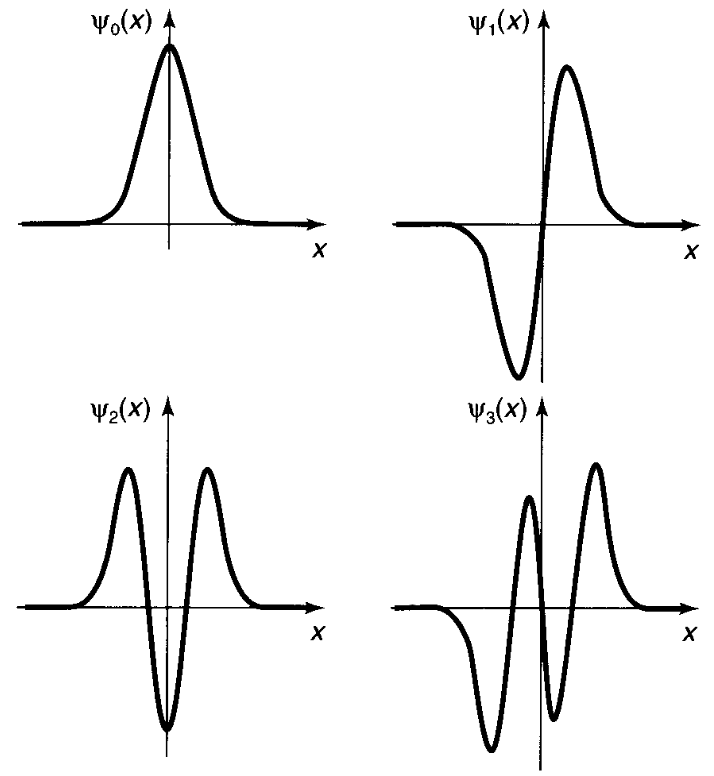
\includegraphics[width=0.6\textwidth]{armonico_func_onda}
    \caption{Primeras funciones de onda para el oscilador armónico}
    \label{fig:armonico_func_onda}
\end{figure}

\subsection{Método algebraico}
Para el método algebraico reescribamos la ecuación de Schrödinger (ecuación \ref{eq:schrodinger_armonico}) de la siguiente forma
\begin{equation}
\frac{1}{2m} \left[\left(\frac{\hbar}{i} \frac{\mathrm{d}}{\mathrm{d}x}\right)^2 + (m \omega x)^2\right]\psi = E\psi
\label{eq:armonico_schrodinger_operador}
\end{equation}

Definimos unos nuevos operadores
\begin{equation}
    a = \frac{1}{\sqrt{2m}} \left(\frac{\hbar}{i} \frac{\mathrm{d}}{\mathrm{d}x} - i m \omega x\right) \qquad 
    a^{\dagger} = \frac{1}{\sqrt{2m}} \left(\frac{\hbar}{i} \frac{\mathrm{d}}{\mathrm{d}x} + i m \omega x\right)
\end{equation}
es decir el operador y su autoadjuto.
También pueden ser.
\begin{equation}
    a = \sqrt{\frac{m \omega}{2 \hbar}} x + i \sqrt{\frac{1}{m \omega \hbar}} \\ a^{\dagger} =  \sqrt{\frac{m \omega}{2 \hbar}} x - i \sqrt{\frac{1}{m \omega \hbar}}
\end{equation}

Estos operadores no son hermíticos, pero si le aplicamos una función cualquiera al producto $a^{\dagger}a$ obtenemos
\[ (a^{\dagger}a) f(x) =  \frac{1}{2m} \left(\frac{\hbar}{i} \frac{\mathrm{d}}{\mathrm{d}x} + i m \omega x\right) \left(\frac{\hbar}{i} \frac{\mathrm{d}}{\mathrm{d}x} - i m \omega x\right) f(x)\]
\[ =  \frac{1}{2m} \left(\frac{\hbar}{i} \frac{\mathrm{d}}{\mathrm{d}x} + i m \omega x\right) \left(\frac{\hbar}{i} \frac{\mathrm{d} f}{\mathrm{d}x} - i m \omega x f\right) \]
\[ =  \frac{1}{2m} \left(- \hbar^2 \frac{\mathrm{d}^2 f}{\mathrm{d}x^2} - \hbar m \omega \frac{\mathrm{d} (x f)}{\mathrm{d}x} + \hbar m  \omega x \frac{\mathrm{d}f}{\mathrm{d}x} + (m \omega x)^2 f\right) \]
\[ = \frac{1}{2m} \left[ \left(\frac{\hbar}{i} \frac{d}{dx}\right)^2 + (m \omega x)^2 - \hbar m \omega\right] f(x) \]
donde usamos regla de la cadena para $\mathrm{d}(x f)/\mathrm{d}x$.
Si eliminamos la función de prueba nos queda
\begin{equation}
    a^{\dagger} a = \frac{1}{2m} \left[\left(\frac{\hbar}{i} \frac{\mathrm{d}}{\mathrm{d}x}\right)^2 + (m \omega x)^2\right] - \frac{\hbar \omega}{2}
\end{equation}
por lo que el hamiltoneano del oscilador queda
\begin{equation}
    (a^{\dagger}a + \frac{1}{2}\hbar \omega) \psi = E \psi
\end{equation}
Si en vez queremos usar el producto $a a^\dagger$ tenemos que la ecuación queda
\begin{equation}
    \left(a a^{\dagger} - \frac{\hbar \omega}{2} \right)\psi = E \psi
\end{equation}
El paso crucial consiste en demostrar que si $\psi$ verifica la ecuación de Schrödinger con energía $E$, entonces $a^{\dagger} \psi$ la verifica con $(E + \hbar \omega)$
\[ (a^{\dagger} a + \frac{\hbar\omega}{2} \psi) (a^{\dagger} \psi) = a^{\dagger} (a a^{\dagger} + \frac{\hbar\omega}{2}) \psi = a^{\dagger} \left[\left(a a^\dagger - \frac{1}{2}\hbar \omega \right)\psi - \hbar \omega \psi \right] = a^{\dagger} (E \psi + \hbar\omega \psi) = (E + \hbar \omega)(a^{\dagger}\psi) \]

Con esto podemos llamar al operador $a^{\dagger}$ como operador de creación o de subida, y al operador $a$ como operador de destrucción o de bajada.

Exigimos ahora la existencia de un estado con energía mínima, tal que si le aplicamos el operador de bajada
\begin{equation}
    a \psi_0 = \frac{1}{2m} \left[\frac{\hbar}{i} \frac{\mathrm{d}\psi_0}{\mathrm{d}x} - i m \omega x \psi_0 \right] = 0
\end{equation}
que se puede resolver por simple integración en
\begin{equation}
    \psi_0 = A_0 e^{-\frac{m \omega}{2\hbar} x^2}
\end{equation}
con autoenergía
\begin{equation}
    E_0 = \frac{\hbar\omega}{2}
\end{equation}

Definido la función de onda del fundamental las siguientes funciones de onda serán
\begin{equation}
    \psi_n(x) = \left(\frac{m \omega}{\pi \hbar}\right)^{1/4} \frac{(-i)^n}{\sqrt{n!(\hbar \omega)^n}} (a^\dagger)^n e^{-\frac{m \omega}{2\hbar} x^2}
\end{equation}
con energía
\begin{equation}
    E_n = \left(n + \frac{1}{2}\right) \hbar \omega
\end{equation}

Y si definimos el operador número
\begin{equation}
    N = a^\dagger a
\end{equation}
con la siguiente propiedad
\begin{equation}
    N |n\rangle = n |n\rangle \qquad \langle x | n \rangle = \psi_n(x)
\end{equation}
por lo que el hamiltoneano queda
\begin{equation}
    H = \hbar \omega \left(N + \frac{1}{2}\right)
\end{equation}

Definamos los conmutadores de los operadores de subida y bajada.
Antes hagamos el cambio de variable con $\xi$
\begin{equation}
    a = \frac{1}{\sqrt{2}} \left[ \xi + \frac{\mathrm{d}}{\mathrm{d}\xi} \right] \qquad a^{\dagger} = \frac{1}{\sqrt{2}} \left[ \xi - \frac{\mathrm{d}}{\mathrm{d}\xi}\right]
\end{equation}
Con esto nos queda
\[ [a,a^\dagger] = a a^\dagger - a^\dagger a = \frac{1}{2} \left[ \left(\xi + \frac{\mathrm{d}}{\mathrm{d}\xi} \right) \left(\xi - \frac{\mathrm{d}}{\mathrm{d}\xi} \right) - \left(\xi - \frac{\mathrm{d}}{\mathrm{d}\xi}\right) \left( \xi + \frac{\mathrm{d}}{\mathrm{d}\xi} \right)\right] = \frac{\mathrm{d}}{\mathrm{d}\xi} (\xi) - \xi \frac{\mathrm{d}}{\mathrm{d}\xi}\]
si se lo aplicamos a una función de $\xi$ cualquiera obtenemos la función nuevamente, por lo que
\begin{equation}
    [a, a^{\dagger}] = 1
\end{equation}

Esto nos permite encontrar que
\[ a^\dagger a a^\dagger |n\rangle =  a^\dagger (a a^\dagger) |n \rangle = a^\dagger (a a^\dagger - a^\dagger a + a^\dagger a) |n \rangle = a^\dagger (1 + n) |n\rangle = (n + 1) a^\dagger |n\rangle\]
Que es lo que ya vimos con el operador de subida, pero deducido solamente con el conmutador.

Los operadores $a$ y $a^\dagger$ no son hermíticos y ni siquiera son diagonales, ya que (mediante normalización)
\begin{equation}
    a^\dagger |n \rangle = \sqrt{n + 1} |n + 1\rangle \qquad a|n\rangle = \sqrt{n} |n - 1\rangle
\end{equation}

\section{Momento angular}

El momento angular en mecánica cuántica se define a partir de la definión clásica
\begin{equation}
    \hat{\boldsymbol{L}} = \hat{\boldsymbol{r}} \times \hat{\boldsymbol{p}} = \frac{\hbar}{i} \hat{\boldsymbol{r}} \times \hat{\nabla}
    \label{eq:momento_angular_def}
\end{equation}
Si definimos al producto vectorial con el simbolo de Levi Civita tenemos
\begin{equation}
    \hat{L}_i = \frac{\hbar}{i} \epsilon_{i j k}  \hat{r}_j \hat{p}_k
\end{equation}

Con la expresión anterior calculemos el conmutador entre componentes del momento angular
\[ [\hat{L}_i, \hat{L}_j] = [\epsilon_{i k l} \hat{r}_k \hat{p}_l, \epsilon_{j m n} \hat{r}_m \hat{p}_m] =  \epsilon_{i k l} \epsilon_{j m n} [\hat{r}_k \hat{p}_l, \hat{r}_m \hat{p}_n] = \epsilon_{i k l} \epsilon_{j m n} ([\hat{r}_k,\hat{r}_m \hat{p}_n] \hat{p}_l + \hat{r}_k [\hat{p}_l, \hat{r}_m \hat{p}_n]) \]
\[ = \epsilon_{i k l} \epsilon_{j m n} (\hat{r}_m [\hat{r}_k, \hat{p}_n]        \hat{p}_l + \hat{r}_k [\hat{p}_l, \hat{r}_m] \hat{p}_n) = \epsilon_{i k l} \epsilon_{j m n} (i \hbar \delta_{k n} \hat{r}_m \hat{p}_l + i \hbar \delta_{l m} \hat{r}_k \hat{p}_n) \] 
\[ = i \hbar \epsilon_{i k l} (\epsilon_{j m l} \hat{r}_m \hat{p}_l + \epsilon_{j l n}  \hat{r}_k \hat{p}_n) = i \hbar (\epsilon_{l i k} \epsilon_{l j m} \hat{r}_m \hat{p}_l + \epsilon_{l i k} \epsilon_{l j m} \hat{r}_k \hat{p}_n)\] 
Si usamos que 
\begin{equation}
    \epsilon_{ijk} \epsilon_{imn}=\delta_{j m} \delta_{kn} - \delta_{jn} \delta_{km}
\end{equation}
llegamos que
\begin{equation}
    [\hat{L}_i, \hat{L}_j] = i \hbar \epsilon_{i j k} L_k
\end{equation}


Defino el operador $\hat{\boldsymbol{L}}^2$ como
\begin{equation}
    \hat{\boldsymbol{L}}^2 = \hat{L}^2_x+\hat{L}^2_y+\hat{L}^2_z = \hat{L}_i \hat{L}_i
\end{equation}
y calculo el conmutador con alguna componente
\[ [\hat{L}_i, \hat{\boldsymbol{L}}^2] = [\hat{L}_i, \hat{L}_j \hat{L}_j] = \hat{L}_j [\hat{L}_i, \hat{L}_j] + [\hat{L}_i, \hat{L}_j] \hat{L}_j = i \hbar (\epsilon_{i j k} \hat{L}_j \hat{L}_k + \epsilon_{i j k} \hat{L}_k \hat{L}_j)\]
ergo
\begin{equation}
    [\hat{L}_i, \hat{\boldsymbol{L}}^2] = 0
\end{equation}

Ahora con la definición del momento angular (ecuación \ref{eq:momento_angular_def}) y la expresión del vector posición y el gradiente en esféricas tengo que
\begin{equation}
    \hat{\boldsymbol{L}} = \frac{\hbar}{i} \left[ \boldsymbol{\phi} \frac{\partial}{\partial \theta} - \boldsymbol{\theta} \frac{1}{\sen(\theta)} \frac{\partial}{\partial \phi} \right]
\end{equation}
del cual podemos deducir que la componente $\hat{L}_z$ es
\begin{equation}
    \hat{L}_z = \frac{\hbar}{i} \frac{\partial}{\partial \phi}
\end{equation}

Lo mismo podemos hacer para el operador $\hat{\boldsymbol{L}}^2$, usando la parte angular del laplaciano $\nabla^2$
\begin{equation}
\hat{\boldsymbol{L}}^2 = - \hbar^2  \left[ \frac{1}{\sen(\theta)} \frac{\partial}{\partial \theta} \left(\sen(\theta \frac{\partial}{\partial \theta} \right) + \frac{1}{\sen^2(\theta)} \frac{\partial^2}{\partial \phi^2} \right]
\end{equation}

\subsection{Método algebraico}

Ahora construyamos dos operadores, de subida y bajada
\begin{equation}
    \hat{L}_{\pm} = \hat{L}_x \pm i \hat{L}_y
\end{equation}
que naturalmente conmuta con $\hat{\boldsymbol{L}}^2$
\begin{equation}
    [\hat{\boldsymbol{L}}^2, \hat{L}_\pm] = 0
\end{equation}
y el conmutador con $\hat{L}_z$ es
\[ [\hat{L}_z, \hat{L}_\pm ] = [\hat{L}_z, \hat{L}_x] \pm i [\hat{L}_z, \hat{L}_y] = i\hbar \hat{L}_y \pm i (-i\hbar \hat{L}_x) = \pm \hbar (\hat{L}_x \pm i \hat{L}_y)\]
es decir
\begin{equation}
    [\hat{L}_z, \hat{L}_\pm ] = \pm \hbar \hat{L}_\pm
\end{equation}

Para completar, podemos ver que la expresión en base de esféricas
\begin{equation}
    \langle \phi, \theta | \hat{L}_\pm | \psi \rangle = - i \hbar e^{\pm i \phi}\left(\pm i \frac{\partial}{\partial \theta} - \cot(\theta) \frac{\partial}{\partial \phi} \right) \langle \phi, \theta | \psi \rangle
    \label{eq:momento_operador_subibda_coordeanas}
\end{equation}

Si tenemos un estado $|\psi\rangle$ tal que
\begin{equation}
    \hat{\boldsymbol{L}}^2 |\psi\rangle = \lambda |\psi\rangle \qquad \hat{L}_z |\psi\rangle = \mu |\psi\rangle
\end{equation}
entonces veamos que produce el operador $\hat{L}_\pm$ a los autoestados del momento angular
\[\hat{\boldsymbol{L}}^2 (\hat{L}_\pm |\psi\rangle = \hat{L}_\pm (\hat{\boldsymbol{L}}^2 |\psi\rangle) = \lambda \hat{L}_\pm |\psi\rangle \]
y para $\hat{L}_z$
\[\hat{L}_z \hat{L}_\pm |\psi\rangle = (\hat{L}_\pm \hat{L}_z - [\hat{L}_z, \hat{L}_\pm]) |\psi\rangle = \hat{L}_\pm (\hat{L}_z \pm \hbar) |\psi\rangle = (\mu \pm \hbar) (\hat{L}_\pm |\psi\rangle) \]

Ahora pedimos que exista un estado superior e inferior tal que
\[ \hat{L}_+ |\psi^f\rangle = 0 \qquad \hat{L}_- |\psi^f\rangle = 0 \]
esos estados tienen los siguientes autovalores
\[ \hat{L}_z |\psi^f\rangle = \hbar l |\psi^f\rangle \qquad \hat{\boldsymbol{L}}^2 |\psi\rangle = \lambda |\psi^f\rangle \]

Para seguir escribimos el operador $\hat{\boldsymbol{L}}^2$ como suma de los otros
\begin{equation}
    \hat{\boldsymbol{L}}^2 = \hat{L}_\pm \hat{L}_\mp + \hat{L}^2_z \mp \hbar \hat{L}_z
\end{equation}

Si se lo aplicamos al estado $|\psi \rangle$ 
\[ \hat{\boldsymbol{L}}^2 |\psi\rangle = (\hat{L}_- \hat{L}_+ + \hat{L}_z + \hbar \hat{L}_z) |\psi\rangle = (0 + \hbar^2 l^2 + \hbar l)|\psi\rangle = \hbar^2 l(l + 1) |\psi\rangle \]

Si hacemos lo mismo para el estado inferior, pidiendo antes que $\hat{L}_z |\psi^b\rangle = \hbar \tilde{l} |\psi^b\rangle$
\[ \hat{\boldsymbol{L}}^2 |\psi^b\rangle = \hbar^2 \tilde{l} (\tilde{l} - 1) |\psi^b\rangle\]

Los autovalores de $\hat{\boldsymbol{L}}^2$ son independientes de los valores de subida y bajada, como ya vimos, por lo que la única solución posible para $l$ es que
\[ \tilde{l} = - l \]
y evidentemente los operadores $\hat{L}_z$ y $\hat{\boldsymbol{L}}^2$ tienen la siguiente propiedad
\begin{equation}
    \hat{L}_z |\psi\rangle = \hbar m |\psi\rangle \qquad \hat{\boldsymbol{L}}^2 |\psi\rangle = \hbar^2 l( l + 1) |\psi\rangle
\end{equation}
con
\begin{equation}
    m \in [-l, l]
\end{equation}
con $N$ valores diferentes de $m$ entre $[-l, l]$, lo que conlleva a decir que $l = -l + N$, con $N = l/2$
\begin{equation}
    l \in \{0, 1/2, 1, 3/2, 2, \dots\} \qquad m \in \{ -l, -l + 1, \dots, l - 1, l\}
\end{equation}

Y los los estados los vamos a escribir como
\begin{equation}
    |\psi\rangle = |l, m\rangle
\end{equation}
si tienen el momento angular definido.

Los operadores de subida y bajada verifican

\begin{equation}
    \hat{L}_\pm |l, m\rangle = \sqrt{l(l + 1) - m( m \pm 1)} |l, m \pm 1
\end{equation}
y la representación en espacio de coordenadas es
\begin{equation}
    \langle \theta, \phi | \hat{L}_\pm |l, m\rangle = \hbar e^{\pm \phi} \left(\pm \frac{\partial}{\partial \theta} + i \cot(\theta) \frac{\partial}{\partial \phi} \right) \langle \theta, \phi | l, m\rangle
\end{equation}
que podemos usar para encontrar las autofunciones de $|l,-l\rangle$ y así sucesivamente.

\subsection{Método analítico}

Ahora resolvamos la ecuación 
\begin{equation}
    \hat{\boldsymbol{L}}^2 |l,m\rangle = \hbar^2 l(l + 1) |l, m\rangle
\end{equation}
ergo
\begin{equation}
    \frac{1}{\sen(\theta)} \frac{\partial}{\partial \theta} \left(\sen(\theta) \frac{\partial}{\partial \theta} f(\theta, \phi) \right) + \frac{1}{\sen^2(\theta)} \frac{\partial^2}{\partial \phi^2} f(\theta, \phi) = - l (l + 1) f(\theta, \phi)
\end{equation}
si multiplico $\sen^2(\theta)$ a ambos lados obtengo
\begin{equation}
    \sen(\theta) \frac{\partial}{\partial \theta} \left(\sen(\theta) \frac{\partial}{\partial \theta} f(\theta, \phi) \right) +  \frac{\partial^2}{\partial \phi^2} f(\theta, \phi) =  -  l (l + 1) \sen^2(\theta) f(\theta, \phi)
    \label{eq:momento_angular_laplace}
\end{equation}

Esta ecuación corresponde a la parte angular de la ecuación de Laplace
\begin{equation}
    \nabla^2 f = \frac{1}{r^2} \frac{\partial}{\partial r}\left( r^2 \frac{\partial f}{\partial r} \right) + \frac{1}{r^2 \sen(\phi)} \frac{\partial}{\partial \phi} \left( \sen(\phi) \frac{\partial f}{ \partial \phi} \right) + \frac{1}{r^2 \sin^2 \phi} \frac{\partial^2 u}{\partial \theta^2} = 0
\end{equation}
con la constante de separación igual a $l(l + 1)$.

Para resolver la ecuación \ref{eq:momento_angular_laplace} proponemos
\begin{equation}
    f(\theta, \phi) = Y_{l m}(\theta, \phi) = \Theta(\theta) \Phi(\phi)
\end{equation}
continuamos dividiendo por $\Theta \Phi$
\begin{equation}
    \left\{ \frac{1}{\Theta} \sen(\theta) \frac{\mathrm{d}}{\mathrm{d}\theta} \left(\sen(\theta) \frac{\mathrm{d}\Theta}{\mathrm{d}\theta}\right) + l (l + 1) \sen^2(\theta) \right\} + \frac{1}{\Phi} \frac{\mathrm{d}^2 \Phi}{\mathrm{d}\phi^2} = 0
\end{equation}
que podemos resolver nuevamente por separación con la constante $m^2$
\begin{equation}
    \begin{gathered}
    \sen(\theta) \frac{\mathrm{d}}{\mathrm{d}\theta} \left(\sen(\theta) \frac{\mathrm{d}\Theta}{\mathrm{d}\theta}\right) + [l (l + 1) \sen^2(\theta) - m^2] \Theta = 0 \\ 
    \frac{\mathrm{d}^2 \Phi}{\mathrm{d}\phi^2} = - m^2 \Phi
\end{gathered}
\end{equation}

La parte polar es fácil de resolver
\begin{equation}
    \Phi = e^{i m \phi}
\end{equation}
y si pedimos continuidad 
\begin{equation}
    \Phi(\phi + 2\pi) = \Phi(\phi)
\end{equation}
llegamos a que 
\begin{equation}
    m \in \mathbb{Z}
\end{equation}

Mientras que la parte azimutal tiene como solución 
\begin{equation}
    \Theta(\theta) = A P^{m}_l(\cos(\theta))
\end{equation}
con $P^{m}_l$ los polinomios de Legendre asociados, definidos como
\begin{equation}
    P^{m}_l(x) = (1 - x^2)^{|m|/2} \left(\frac{\mathrm{d}}{\mathrm{d}x}\right)^{|m|} P_l(x)
    \end{equation}
y los polinomios de Legendre los podemos definir con la fórmula de Rodrigues
\begin{equation}
    P_l(x) = \frac{1}{2^l l!} \left(\frac{\mathrm{d}}{\mathrm{d}x}\right)^{l} (x^2 - 1)^l
\end{equation}

Finalmente podemos deducir las reglas para $l$ y $m$ usando que la $n$-esima derivada  de cualquier polinomio de grado $n'$ es nula si $n > n'$
\begin{equation}
    l \in \mathbb{N}^0 \qquad m \in [-l, l], m \in \mathbb{Z}
\end{equation}

Finalmente las funciones normalizadas serán
\begin{equation}
    Y^{m}_l = \epsilon \sqrt{\frac{2l + 1}{4\pi} \frac{(l - |m|)!}{(l + |m|)!}} e^{i m \phi} P^{m}_l(\cos(\theta))
\end{equation}
con $\epsilon = (-1)^m$ si $m \geq 0$ o $\epsilon = 1$ si $m \leq 0$.


\subsection{Rotaciones infinitesimales y sus generadores}

Una función escalar $\phi$ observa el siguiente cambio al rotarse infinitesimalmente un ángulo $\delta \boldsymbol{\varphi}$
\begin{equation}
    \delta \phi = -\frac{i}{\hbar} \delta \boldsymbol{\varphi} \dot \hat{\textbf{L}} \phi(\textbf{r})
\end{equation}
indicando que el generador de las rotaciones es el momento angular.

Esto se puede generalizar para cualquier tipo de momento, y además puede ser usado como definición del momento angular y deducir las relaciones de conmutación.

\section{Fuerzas centrales}

Un problema general de fuerzas centrales es
\begin{equation}
    \hat{H} = \frac{\hat{\boldsymbol{p}}^2}{2m} + V(\hat{\boldsymbol{r}})
\end{equation}
con la siguiente represntación en coordenadas esféricas
\begin{equation}
    \langle \boldsymbol{r}|\hat{H}|\psi\rangle = \frac{-\hbar^2}{2m} \nabla^2 \psi(\boldsymbol{r}) + V(\textbf{r}) \psi(\boldsymbol(r)) = E \psi(\textbf{r}) 
\end{equation}

Todo problema de fuerzas centrales tiene la misma parte angular, que ya resolvimos, los armónicos esféricos, y diferente parte radial depediendo de la forma del potencial.

Usando la constante de separación $l (l + 1)$) tenemos que la parte radial $R(r)$ de la función de onda verifica
\begin{equation}
    \frac{\mathrm{d}}{\mathrm{d}r} \left(r^2 \frac{\mathrm{d} R}{\mathrm{d}r} \right) - \frac{2 m r^2}{\hbar^2} (V(r) - E - l(l + 1)) R = 0
\end{equation}

Para resolver esta ecuación proponemos el cambio de variable $u = R/r$
\begin{equation}
    -\frac{\hbar^2}{2m} \frac{\mathrm{d}^2 u}{\mathrm{d}r^2} + \left[ V(r) + \frac{\hbar^2}{2m} \frac{l (l + 1)}{r^2} \right] u = E u
    \label{eq:central_ec_radial}
\end{equation}
que se denomina ecuación radial.


\subsection{Átomo de hidrógeno}
Consideramos la masa del nucleo muy grande o usamos la masa reducida, y el potencial columbiano en unidades gaussianas
\begin{equation}
    V(r) = -\frac{e^2}{r}
\end{equation}

La ecuación radial (ecuación \ref{eq:central_ec_radial}) queda
\begin{equation}
    -\frac{\hbar^2}{2m} \frac{\mathrm{d}^2 u}{\mathrm{d}r^2} + \left[ - \frac{e^2}{r} + \frac{\hbar^2}{2m} \frac{l (l + 1)}{r^2} \right] u = E u
\end{equation}
Si ahora rescribimos las constantes con $\kappa = \frac{\sqrt{-2mE}}{\hbar}$ tenemos
\[\frac{1}{\kappa^2} \frac{\mathrm{d}^2 u}{\mathrm{d} r^2} = \left[1 - \frac{m e^2}{2 \hbar^2 \kappa} \frac{1}{\kappa r} + \frac{l (l + 1)}{(\kappa r)^2} \right] u\]

Con el cambio de variables $\rho = \kappa r$ y $\rho_0 = \frac{m e^2}{2 \hbar^2 \kappa}$ tenemos
\begin{equation}
    \frac{\mathrm{d}^2 u}{\mathrm{d}\rho} = \left[1 - \frac{\rho_0}{\rho} + \frac{l(l + 1)}{\rho^2}\right] u
\end{equation}

Para resolver la ecuación anterior veamos el comportamiento para $\rho \to 0$ y para $\rho \to \infty$
\begin{equation}
    \begin{gathered}
        \rho \to 0 \implies \frac{\mathrm{d}^2 u}{\mathrm{d} \rho^2} \approx \frac{l(l + 1)}{\rho^2} u\\
        \rho \to \infty \implies \frac{\mathrm{d}^2 u}{\mathrm{d} \rho^2} = u
    \end{gathered}
\end{equation}

Las soluciones posibles a estas ecuaciones son
\begin{equation}
    \begin{gathered}
        \rho \to \infty  \implies u(\rho) = A e^{-\rho} + B e^{\rho} \\
        \rho \to 0 \implies u(\rho) = C \rho^{l + 1} + D \rho^{-l}
    \end{gathered}
\end{equation}
y si eliminamos las divergencias obtenemos
\begin{equation}
    u(\rho) = \rho^{l + 1} e^{-\rho} v(\rho)
\end{equation}

De esta forma la ecuación para $v(\rho)$, que corresponde a la ecuación radial con el reemplazo de la función de prueba, será
\begin{equation}
    \rho \frac{\mathrm{d}^2 v}{\mathrm{d}\rho^2} + 2(l + 1 - \rho) \frac{\mathrm{d} v}{\mathrm{d}\rho} + [\rho_0 - 2(l + 1)] v = 0
\end{equation}
Si en esta ecuación pruebo una serie de potencia
\begin{equation}
    v(\rho) = \sum_{j = 0}^\infty a_j \rho^j
\end{equation}
y obtenemos una relación de recurrencia calculando las derivadas pertinentes en la ecuación diferencial
\begin{equation}
    a_{j + 1} = \left[ \frac{ 2(j + l + 1) - \rho_0}{(j + 1) (j + 2l + 2)}\right] a_j
\end{equation}
Nuevamente si observamos el comportamiento asintótico de los coeficientes encontramos que debe terminar, es decir que exista un valor para el cual $a_{j + 1} = 0$, que es evidentemente
\begin{equation}
    2 (j_{max} + l + 1) - \rho_0 = 0
\end{equation}
y si definimos 
\begin{equation}
    n = j_{\max} + l + 1
\end{equation}
como un número entero, por lo tanto los valores de $l$ serán
\begin{equation}
    l \in \{0, 1, 2, \dots, n - 1\}
\end{equation}
y además podemos encontrar la energía, sabiendo que 
\[ \rho_0 = \frac{m e^2}{2 \hbar \sqrt{-2 m E}} = 2n\]
por lo que finalmente (recordando que $\kappa = \frac{\sqrt{-2 m E}}{\hbar}$
\begin{equation}
    E = - \frac{m e^4}{2 \hbar^2} \frac{1}{n^2} = \frac{E_1}{n^2}
\end{equation}
que corresponde a la energía encontrada por Bohr años antes de resuelta la ecuación de Schröndinger.

La función $v(\rho)$ es 
\begin{equation}
    v(\rho) = L^{2l + 1}_{n - l -1}(2\rho)
\end{equation}
siendo el simbolo ese
\begin{equation}
    L^{p}_{q - p}(x) = (-1)^p \left(\frac{\mathrm{d}}{\mathrm{d}x}\right)^p L_q(x)
\end{equation}
un polinomios de Laguerre asociado, y
\begin{equation}
    L_q(x) = e^x \left(\frac{\mathrm{d} (e^-x x^q)}{\mathrm{d}x}\right)^q
\end{equation}
los polinomios de Laguerre.

Para completar presentamos las autofunciones normalizadas

\begin{equation}
    \psi_{nlm}(r,\phi,\theta) = \sqrt{\left(\frac{2}{n a}\right)^3 \frac{(n - l - 1)!}{2n[(n + l)!]^3}} e^{-r/(na)} \left(\frac{2r}{na}\right)^l L^{2l + 1}_{n - l - 1}\left(\frac{2r}{na}\right) Y^{m}_{l}(\theta, \phi)
\end{equation}

con $a$ el radio de Bohr
\begin{equation}
    a = \frac{\hbar^2}{m e^2} = 0,529 \times 10^{-10}\;\text{m}
\end{equation}
que corresponde al radio de la primera orbita.
Este radio también se puede encontrar invocando al principio de incertidumbre.

\section{Spin}

En varias experiecias, en particular las de Stern y Gerlach (que se observa en la figura \ref{fig:stern_gerlach}) que demostró la existencia de un momento angular intrínseco al observar un momento dipolar magnético intrínseco.

\begin{figure}[H]
    \centering
    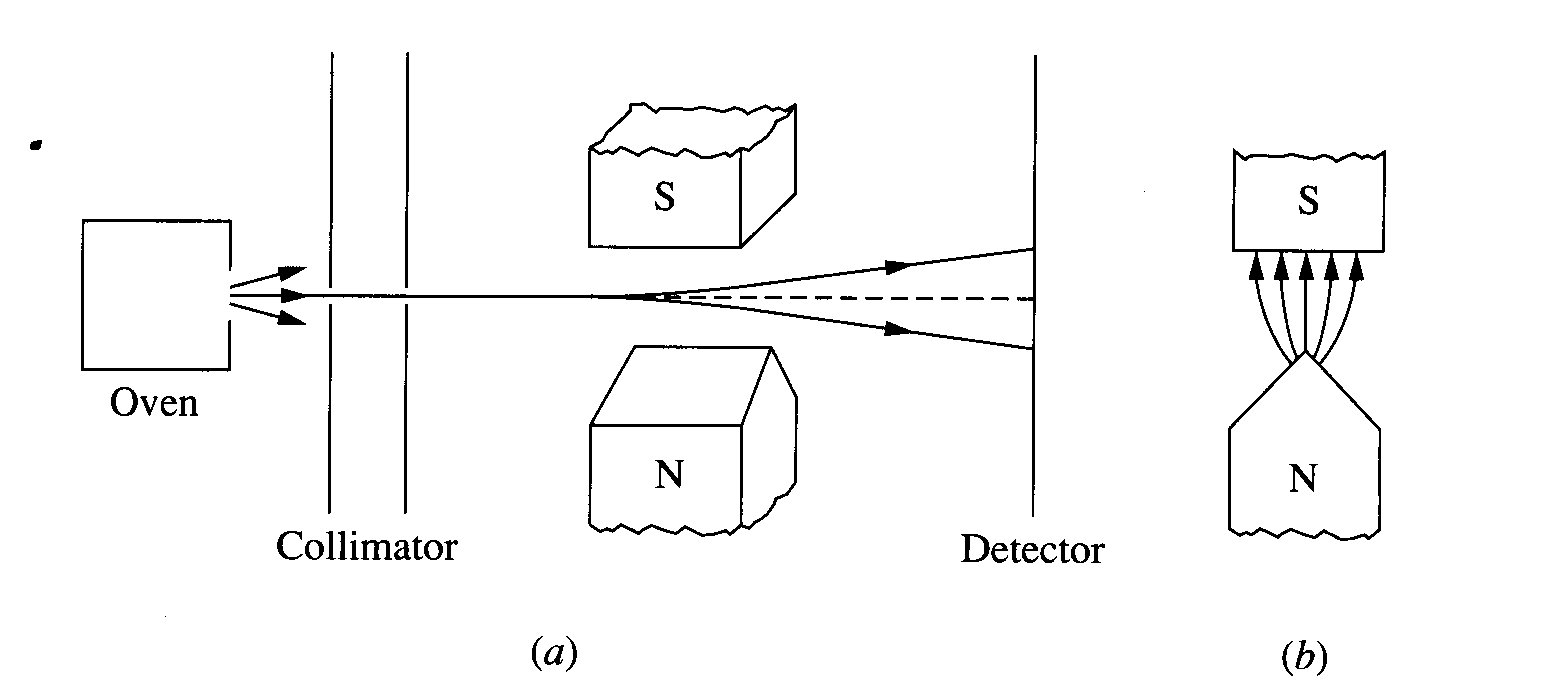
\includegraphics[width=0.5\textwidth]{stern_gerlach}
    \caption{Experimento de Stern Gerlach}
    \label{fig:stern_gerlach}
\end{figure}

Asumido que existe este operador, que llamamos \emph{spin}, podemos usar toda la teoría algebraica del momento angular para explicarlo, empezando con las reglas de conmutación
\begin{equation}
        [\hat{S}_i, \hat{S}_j] = i \hbar \epsilon_{ijk} \hat{S}_k \qquad [\hat{S}_i, \hat{S}^2] = 0
\end{equation}
con lo que podemos deducir que los autoestados de los operadores  son
\begin{equation}
\hat{S}_z |s,m\rangle = \hbar m |s,m\rangle \qquad \hat{S}^2 |s, m\rangle = \hbar^2 s(s + 1) |s,m\rangle
\end{equation}
También agregamos los operadores de subida y bajada
\begin{equation}
 \hat{S}_\pm = \hat{S}_x \pm i \hat{S}_y
\end{equation}
con la siguiente propiedad
\begin{equation}
\hat{S}_\pm |s, m\rangle = \sqrt{s(s+1) - m( m \pm 1)} |s, m \pm 1 \rangle 
\end{equation}

Para el spin de $1/2$, tenemos dos estados
\begin{equation}
    s = \frac{1}{2} \implies |s,m\rangle \in \left\{\left|\frac{1}{2},\frac{1}{2}\right.\rangle, \left|\frac{1}{2},-\frac{1}{2}\right.\rangle\right\}
\end{equation}
Estos estados los podemos expresar en forma matricial como
\begin{equation}
|1/2,1/2\rangle = \begin{pmatrix} 1 \\ 0 \end{pmatrix} \qquad |1/2,-1/2\rangle = \begin{pmatrix} 0 \\ 1 \end{pmatrix}
\end{equation}
Un estado general se puede expresar por lo tanto
\begin{equation}
    \xi = \begin{pmatrix} a \\ b \end{pmatrix}
\end{equation}
Estos elementos de matrix se denomina espinores, porque al rotarlos $2\pi$ cambian de signo (usando la rotación inducida por el operador $\hat{\boldsymbol{S}}$).

Si escribimos los operadores $\hat{S}_i$ y $\hat{S}^2$ con esta notación obtenemos
\begin{equation}
    \begin{gathered}
        \hat{S}_z = \frac{\hbar}{2} \begin{pmatrix} 1 & 0 \\ 0 & -1 \end{pmatrix} \qquad
        \hat{S}_x = \frac{\hbar}{2}\begin{pmatrix} 0 & 1 \\ 1 & 0 \end{pmatrix}\\ 
    \hat{S}_y = i \begin{pmatrix} 0 & -1 \\ 1 & 0 \end{pmatrix} \qquad
    \hat{S}^2 = \frac{3}{2}\hbar \begin{pmatrix} 1 & 0 \\ 0 & 1 \end{pmatrix}
\end{gathered}
\end{equation}
Las matrices de $\hat{S}_x$ y $\hat{S}_y$, que las encontramos usando las expresiones de $\hat{S}_\pm$, son diagonales en los siguientes estados
\begin{equation}
    \begin{gathered}
    \hat{S}_x \text{ es  diagonal en } \left\{\frac{|+ \rangle + i |-\rangle}{\sqrt{2}}, \frac{|+\rangle - i |-\rangle}{\sqrt{2}}\right\} \\
    \hat{S}_y \text{ es  diagonal en } \left\{\frac{|+\rangle + |-\rangle}{\sqrt{2}}, \frac{|+\rangle - |-\rangle}{\sqrt{2}}\right\}
\end{gathered}
\end{equation}

Estas matrices son conocidas como de Pauli, y las matrices $\hat{S}_i$ y $\hat{S}^2$ son hermíticas (y observables), pero no así las $\hat{S}_\pm$
Lo mismo podemos hacer para spin de más dimensiones, lo único es necesario recordar la expresión de los operadores $\hat{S}_\pm$.
Acá se vuelve a mostrar la utilidad de este método con operadores.

\section{Estadísticas cuánticas}
  Los bosones (spin entero) exigen función de onda simétrica 
\begin{equation}
  P |\psi\rangle = |\psi\rangle
\end{equation}
mientras los fermiones (spin semientero) exigen
\begin{equation}
 P |\psi\rangle = - |\psi\rangle
\end{equation}
es decir función de onda antisimétrica
Dadas $n$ partículas con estados $|\psi_i(\alpha_i)\rangle$ (donde $\alpha_i$ es un parámetro del estado, como la posición), para construir el estado más general de fermiones tenemos el determinante de Slatter
\begin{equation}
  |\psi\rangle = \frac{1}{\sqrt{n}} \begin{vmatrix} |\psi_1(\alpha_1)\rangle & |\psi_2(\alpha_1)\rangle & \cdots & |\psi_n(\alpha_1)\rangle \\  |\psi_1(\alpha_2)\rangle & |\psi_2(\alpha_2)\rangle & \cdots & |\psi_n(\alpha_2)\rangle \\ \vdots & \vdots & \ddots & \vdots \\  |\psi_1(\alpha_n)\rangle & |\psi_2(\alpha_n)\rangle & \cdots & |\psi_n(\alpha_n)\rangle \end{vmatrix}
\end{equation}
y para bosones usamos el permanente de la matriz, como si fuese un determinante pero sin alternar los signos
\begin{equation}
   |\psi\rangle = \frac{1}{\sqrt{n}}\; \text{perm}\begin{pmatrix} |\psi_1(\alpha_1)\rangle & |\psi_2(\alpha_1)\rangle & \cdots & |\psi_n(\alpha_1)\rangle \\  |\psi_1(\alpha_2)\rangle & |\psi_2(\alpha_2)\rangle & \cdots & |\psi_n(\alpha_2)\rangle \\ \vdots & \vdots & \ddots & \vdots \\  |\psi_1(\alpha_n)\rangle & |\psi_2(\alpha_n)\rangle & \cdots & |\psi_n(\alpha_n)\rangle \end{pmatrix}
\end{equation}



\end{document}

